\documentclass[10pt]{scrreprt}

% quick TOC setup
\KOMAoption{toc}{chapterentrydotfill}
% don't use parskip package, set parskip=full instead
\KOMAoption{parskip}{half}

\usepackage[twoside
            ,papersize={148mm, 210mm}
            ,layoutsize={148mm, 210mm}
            ,top=1.5cm
            ,bottom=2cm
            ,footskip=1cm
            ,textwidth=12cm
            ,verbose
            ]{geometry}

% \renewcommand*{\chapterheadstartvskip}{}

\usepackage[english]{babel}

\usepackage{graphicx}
\usepackage{fancyhdr}
\usepackage{eso-pic}
\usepackage{caption}
\usepackage{wrapfig}
\usepackage{menukeys}
\usepackage{amssymb}
\usepackage{eurosym}
\usepackage{multicol}
\usepackage{lscape}
\usepackage{comment}
\setlength{\multicolsep}{0.5em}
\usepackage{adjustbox}
% fancy fone awesome boxes
\usepackage{awesomebox}

% mainly for linklist
\usepackage{longtable}
\usepackage{enumitem} % to easily remove itemize indent for the checklist

\usepackage{pdfpages}
\usepackage{fontspec}
\usepackage{microtype}
\usepackage[autostyle=true]{csquotes}

\PassOptionsToPackage{hyphens}{url}
\usepackage[colorlinks=false, pdfborder={0 0 0}]{hyperref}
\hypersetup{
	pdfauthor={FSR Informatik der TU Dresden},
	pdftitle={The Manual - ESE 2022},
	breaklinks=true, colorlinks=false, pdfborder={0 0 0},
  pdfencoding=unicode
}


% \definecolor{ese_bg_color}{rgb}{0.0, 0.20, 0.376} % the definitive color -- #003360 (2015?)
% \definecolor{ese_bg_color}{rgb}{0.0, 0.263, 0.486} % the definitive color -- #00437C (2016?)
% \definecolor{ese_bg_color}{rgb}{0.051, 0.373, 0.596} % the definitive color -- #0D5F98 (2017)
% \definecolor{ese_bg_color}{rgb}{0.796, 0.376, 0.251} % the definitive color -- #CB6040 (2018)
% \definecolor{ese_bg_color}{rgb}{0.0, 0.47, 0.3} % wip-ish color -- #01794C (2019)
% \definecolor{ese_bg_color}{RGB}{5,109,133} % final_really_final -- #056d85 (2020)
\definecolor{ese_bg_color}{RGB}{155,30,70} % complement -- #9B1E46 (2021)
\definecolor{ese_fg_color}{rgb}{1, 1, 1}

\definecolor{fancypageref_color}{RGB}{155,30,70} % 

\definecolor{ifsrgray}{rgb}{0.6, 0.6, 0.6} % 153, 153, 153

% is toggled twice for moduluebersicht.tex
\changemenucolor{gray}{bg}{named}{ese_fg_color} %background of the menukeys
\changemenucolor{gray}{br}{named}{ese_bg_color} %border of the menukeys
\changemenucolor{gray}{txt}{named}{ese_bg_color} %text of the menukeys

\setmainfont[
  Scale=0.90,
  BoldFeatures={Scale=1.0}
]{Open Sans}

\setmonofont[
	Scale = 1.09
]{Latin Modern Mono}

\setkomafont{chapter}{\color{ese_bg_color}\fontspec[BoldFont={* Bold}]{Open Sans}\huge\bfseries}
\setkomafont{minisec}{\color{ifsrgray}\fontspec[BoldFont={* Bold}]{Open Sans}\large\bfseries}
\setkomafont{paragraph}{\color{ifsrgray}\fontspec[BoldFont={* Bold}]{Open Sans}}
\setkomafont{pagenumber}{\color{ifsrgray}\fontspec{Open Sans}}

\addtokomafont{disposition}{\normalfont\fontspec{Open Sans}}
\defaultfontfeatures{Ligatures=TeX}  % enable ligatures (e.g. --) for new fonts

\newcommand{\ascii}{{\texttt{ascii}}}


% we need this dummy counter to make a label at the spieleabendplakat
\newcounter{dummy}

\newcounter{linkcounter}
\newcommand\linklist{}
\renewcommand{\minisec}[1]{\subsection*{#1}}
\makeatletter
\def\@breaklinklistat{22}
\def\@breaklinklistandat{54}

\makeatother

\sloppy % forces "ugly" line breaks

\pagestyle{plain}

\def\link#1{\url{#1}}

\begin{document}

\tableofcontents

%\textit{\foreignlanguage{english}{\enquote{Any inaccuracies in this index may be explained by the fact that it has been sorted with the help of a computer.}}}\\
%\mbox{}\hfill --- Donald Knuth

% Wie erstellt man den Zeitplan?
% 1. man läd sich den HTML Code von ese.ifsr.de herunter
% 2. man fügt folgendes CSS manuell hinzu und bestaunt das Ergebnis:
%  *{font-size:0.99!important}
%	main {margin:0;padding:0;}
%	.row {margin:0;}
%	 header, footer, .sidebar, .panel, section h2, section p, #barrierfree-heading, #timetable-heading  {display:none;}
%	tr, td  {line-height: 1em;}
%	table tbody tr td div.table-spacer {height: 1rem;!important}
%	#content {padding:0;}
%
%	td.data {width: 20%; background: #FDC412}
% 3. man benutzt z.B. wkhtmltopdf um ein PDF daraus zu erstellen:
% wkhtmltopdf -s A4 --no-print-media-type --margin-left 0 --margin-right 0 --margin-bottom 0 --margin-top 0 ESE\ 2016\ _\ iFSR.html zeitplan.pdf
% 4. ????
% 5. Färdsch
%  \vspace*{-6.5em}
\thispagestyle{empty}

\chapter*{Timetable}

The current time table is available at \url{https://ese.ifsr.de/}.

%
%  Sofern nicht anders angegeben, finden alle Veranstaltungen im Fakultätsgebäude der Informatik, dem
%  \textbf{Andreas Pfitzmann Bau (APB)}, im Raum \textbf{E023} (Hörsaal direkt am Foyer) statt.
%  Folge im Gebäude einfach den vielen Tutoren in den schönen, roten ESE-2018-Shirts.
%

\chapter{What is this?}

Hello! You've already made it this far. Wow!

As you might find out in the course of your now beginning studies, 
one of the hardest tasks is to get a computer scientist to read the manual or the documentation. 
Maybe it's a quirk we have, or maybe we just prefer to tinker with a problem for days on end rather than spend half an hour looking it up in the manual. 
That's why you'll often hear the phrase: \enquote{RTFM} -- Read the fucking manual -- 
in forums or on \href{https://stackoverflow.com/}{StackOverflow}.

But the good news is, if you are reading this, you are already counteracting this prejudice. 
Because this booklet is a small manual for your studies. It tells you how the university works, how courses are structured, how to register for exams, what the campus has to offer and much more. 

% Like any good handbook, it contains far too much information that you can hardly use or process at once.

% That's why it's enough to read only the chapters marked with \keys{must read} 
% and look up the rest later or use the FAQ section on page \pageref{sec:faq} to find the right answers. 

This book is designed to help you with information and answers throughout most of your studies. 
So keep it and take it out every now and then. Like every good handbook :)

And now away with the book! The Erstsemestereinführung (ESE) is waiting for you, which will explain the most important things to you in the coming week. Enjoy this time and get ready for the even more exciting one that awaits you now!

\textbf{All that remains is to say: Enjoy the ESE and your studies!}

% Martin, 31. August 2022
% In dem Handbuch sollten einfach nur die wichtigsten Dinge genau einmal stehen (DRY), 
% damit man es einfach einmal lesen kann.

\chapter{Greeting}


\includegraphics[width=0.3\textwidth]{img/sbalzarini.jpg}


Dear Students,

a wholehearted \enquote{Welcome} to the Faculty of Computer Science at TU Dresden! Congratulations for having decided to study computer science our university, as no other course of studies would nowadays open so many doors and provide you with so many opportunities like ours, and TU Dresden provides you with an excellent environment to pursue your goals in one of Germany’s most livable and affordable student cities.

We are a diverse, international, and interdisciplinary community of about 2400 students (every third from abroad), 220 scientists, 222 registered PhD students, 28 professors, 4 Honorary Professors, and two independent Group Leaders with the status of \enquote{TUD Young Investigator}. Together, we are one of the top computer science departments in Germany. We offer a selection of nine degree programs, including two international Master’s programs entirely taught in English. These curricula cover the entire breadth of our exciting discipline. And we are fortunate to do so under excellent conditions with state-of-the-art infrastructure. Our department is housed in a modern building offering generous teaching rooms and well-equipped labs. We have access to some of the best high-performance computing resources of Germany with machines hosted in a dedicated building just next door. Finally, our university's sports facilities are located just behind our building, and the student-run café \ascii{} in the Lobby of our building is a focal point of our social life.

Our building is proudly named after Prof. Andreas Pfitzmann, who was our chair of privacy and security until 2010. Andreas Pfitzmann's work was not only scientifically noted, but his social engagement had far-reaching consequences for the public opinion and the lawmaking in Germany. Andreas Pfitzmann is partly responsible for the fact that the German public has an internationally unparalleled level of awareness when it comes to topics of data protection, security, and privacy.  This is just one example of how computer science directly impacts and shapes many areas of our everyday lives. A young discipline, computer science is unique in its blend of being both a structural science, like mathematics and philosophy, and an engineering discipline. It has revolutionized the way we communicate with each other, the way we run organizations, manage industrial production, and do science in almost all disciplines. There is almost no area of science, technology, or society that would not be shaped by and depend on advancements in computer science. Computing is a universal language that reaches far beyond tech geekery and hobbyist programming. It is theory and algorithms that provide a rigorous mathematical understanding of "information processing". It is human-machine interaction and the human in the loop, linking our discipline to psychology and the arts. It is the information processing that happens in living cells and organisms by chemical signaling pathways and the neurons in our brains, linking to systems biology and medicine. It is machine learning and artificial intelligence that aim to produce \enquote{thinking machines}. It is data security and privacy with all its connections to the mathematics of cryptography, systems engineering, as well as societal and legal aspects. It is embedded systems, robotics, smart and autonomous systems with connections to electrical and mechanical engineering. Computer science is everywhere, and our faculty collaborates with pretty much every other department of TU Dresden, from medicine and environmental science, to mechanical and electrical engineering, to psychology and law in order to contribute toward solving humankind’s most challenging problems.

No wonder that computer science in Dresden is growing rapidly. Our faculty is set to enlarge with additional professorships, e.g., in the areas of data science and artificial intelligence. We have been extraordinarily successful in winning competitive national centers: We are hosting one of the nine National High-Performance Computing Centers (NHR) of Germany, one of the five Federal Centers for Machine Learning and AI, the ScaDS.AI Dresden/Leipzig, one of the four Centers for the next generation of mobile communication, 6G-Life, and one of only three DAAD Zuse Schools of Excellence in AI (SECAI). We are also a major partner in two DFG Clusters of Excellence (the Center for Tactile Internet, CeTI, and the Center for the Physics of Life, PoL), and we participate in the only Else-Kröner-Fresenius Center for Digital Health (EKFZ) in Germany. I am convinced you will benefit from the presence of these internationally visible top research and teaching centers with their unparalleled computational and academic infrastructure. 

Beyond our university, you will also benefit from the unique DRESDEN-concept alliance that the TU Dresden has founded with 32 non-university research institutions in our city. Dresden has been named as a city of Science in 2006 and has attracted an impressive number and concentration of research organizations. All major players are here with several institutes each: the Max Planck Society, the Helmholtz Association, the Fraunhofer Society, and the Leibniz Association, in addition to many research-active museums, hospitals, and cultural organizations. Under the common umbrella of DRESDEN-concept e.V., they greatly enrich your freedom of choice in finding exciting topics for your project modules, Bachelor's, Master's or Diplom thesis, or to stay on for a PhD after graduation. 

And if a PhD is not for you, then there are ample job opportunities in the IT industry in and around Dresden. The Saxon IT sector has been steadily growing by 5 to 7 \% per year since the German reunification. In Dresden alone, jobs for 600 to 800 computer science graduates are created each year. And this trend is set to further accelerate, as large multi-national corporations continue to move into our city. Some of them moved here specifically because of our degree programs and graduates,  that is because of you!

But first, you need to successfully master your studies. And that will be challenging. It is through challenges that we grow, as they say. So please consider the challenges you are undoubtedly going to meet in the coming semesters as such: challenges to grow on, not problems. A university is not a school. Many things are not predefined, there is a lot of freedom from designing your curriculum to deciding where to look for project topics. Welcome to the land of plenty! Benefit from the freedom and diversity of topics offered, but work systematically and diligently in order to not get lost in the multitude of possibilities. And if you do happen to get a bit lost, then please take advantage of the many counseling and mentoring offerings we provide for students. Work on developing your ability to learn independently and, most importantly, on your ability to judge yourself realistically. It is an easy trap to fool yourself into believing you have understood, and it is hard to know for sure when you actually did. Talking to others and actively and independently doing the exercises and homework is paramount to success. In a university, many problems are not "presented" to you, but you are expected to independently identify them. Likewise, you will be increasingly expected to be able to decide for yourself if one of your solutions is correct or not. Most people do not pass exams by simply sitting through lectures or reading a book. It is only through learning by doing in the exercises and tutorials that you achieve the ability to transfer knowledge to previously unseen problems. 

And for this journey of personal development, I wish you all the best of success! And of course fun. You will learn many fun things here and find many courses offered to you free of charge to satisfy your thirst for knowledge. Do not focus on the outcome, but enjoy the process! And do not hesitate to talk to us and become an active member of our community. Get engaged with the student association iFSR, find your network of friends and peers among the other students, ask senior students and tutors for advice, and do not hesitate to talk to your professors if you have questions or require help. We live a culture of open doors and wish to make your student experience here as rewarding and productive as possible. Probably the best example for this is the ESE, our welcome week for new students, which you are starting right now. The ESE is entirely student-organized, run by our student association, and financially supported by the faculty and by external sponsors. Big thanks to the iFSR and the sponsors! And now, dive in and enjoy the ride! Many exciting new things are awaiting you on your journey to becoming part of the global computer science community that shapes our future. 

   SHAPE YOUR FUTURE!

\textit{Ivo F. Sbalzarini,\\
Dean of the Faculty of Computer Science }

\chapter*{Frequently Asked Questions}
\addcontentsline{toc}{chapter}{Frequently Asked Questions \hspace*{.1cm} \keys{must read}}
\label{sec:faq}
\minisec{Was muss ich während des Semesters machen?}
Prinzipiell nichts außer dich am Ende zurückzumelden, um weiter immatrikuliert zu sein.

\minisec{Was sollte ich während des Semesters machen?}
Du solltest die Übungen und Vorlesungen besuchen, um am Ende die Prüfungen zu bestehen.

\minisec{Wie schreibe ich mich in Prüfungen ein?}
Für die schriftlichen Prüfungen in den Pflichtmodulen läuft die Anmeldung über jExam~\link{https://jexam.inf.tu-dresden.de/}.
Dort gibt es am Ende der Vorlesungszeit eine Liste mit allen Prüfungen, in die du dich einschreiben kannst.

\minisec{Wie kann ich mich von Prüfungen abmelden?}
Du kannst dich ohne Angabe von Gründen bis drei Werktage von schriftlichen Prüfungen über jExam abmelden. Falls du erkrankt bist, kannst du auch noch danach von der Prüfung zurücktreten. Der Krankenschein ist dann dem Prüfungsamt zügig vorzulegen.

\minisec{Ich habe eine Prüfung nicht bestanden, wann muss ich sie wiederholen?}
Nicht-bestandene Modulprüfungen müssen innerhalb eines Jahres einmal wiederholt werden. Beim Nichtbestehen muss eine zweite Wiederholung zum nächstmöglichen Prüfungstermin abgelegt werden. Danach gilt die Modulprüfung endgültig als nicht bestanden. 
Durch COVID-19 kann es sein, dass es Sonderregulungen diesbezüglich gibt. Hier gilt es, sich stehts informiert zu halten z.B. auf der Corona-Informationsseite der TU Dresden \link{https://tu-dresden.de/tu-dresden/gesundheitsmanagement/information-regarding-covid-19-coronavirus-sars-cov-2}. 
Übrigens: Eine aus mehreren Prüfungsleistungen bestehende Modulprüfung kann bei entsprechender Gewichtung der Noten bestanden sein, auch wenn eine der Prüfungsleistungen nicht bestanden ist.

\minisec{Wie lange darf man überhaupt studieren?}
In Kurzform: Regelstudienzeit + 4 Semester. Es gibt aber einige Möglichkeiten, wie z.B. Urlaubs- und Gremiensemester, um diese Dauer zu verlängern. Bedenke aber, dass ab dem 14. Fachsemester Langzeitstudiengebühren fällig werden.

\minisec{Wie baue ich mir meinen Stundenplan?}
Für den Anfang bekommst du fertige Stundenpläne von uns, aus denen du dann einfach einen Stundenplan am Tag der Einschreibung auswählen kannst. Ab dem zweiten Semester bieten die Studienablaufpläne eine Empfehlung, welche Module man in welchem Semester besuchen sollte. Du suchst dir die Lehrveranstaltungen aus dem Katalog aus, die du besuchen möchtest. Dann suchst du dir Termine heraus und versuchst, Kollisionen zu vermeiden.

\minisec{Was ist AQua?}
Diese Abkürzung steht für Allgemeine Qualifikation. Es ist ein Bestandteil deines Studiums~\fancypageref{lec:aqua}.

%\minisec{Was sollen diese ganzen Portale?}
%In guter Tradition gibt es für jeden Zweck mindestens 5 verschiedene Portale. Das muss so. Für dich sind eigentlich nur folgende wichtig:
%\begin{itemize}
%\item jExam für die Einschreibung in Lehrveranstaltungen und Prüfungen
%\item Selma~\link{https://selma.tu-dresden.de} für das Herunterladen der Immatrikulationsbescheinigung
%\item OPAL wird besonders in der Online-Lehre häufig für die Einschreibung und Organisation von Lehrveranstaltungen genutzt.
%\end{itemize}

\minisec{Wie funktioniert das mit dem WLAN?}
Das ZIH hat Anleitungen~\link{https://tu-dresden.de/zih/dienste/service-katalog/arbeitsumgebung/zugang_datennetz/wlan-eduroam} für viele Systeme zum Einrichten des Eduroam. Falls die Anleitungen dein Problem nicht lösen, hilft dir der ServiceDesk weiter.

\minisec{Was muss ich tun, um BAföG zu bekommen?}
Das Studierendenwerk~\fancypageref{sec:stuwe} ist für die Bearbeitung der Anträge zuständig und bietet auch entsprechende Beratung an. Daneben kannst du dich mit deinen Fragen auch an den StuRa~\fancypageref{sec:stura} wenden.

\minisec{Wie und wann melde ich mich für Unisport an?}
Das funktioniert über das Universitätssportzentrum, das alle Kurse verwaltet~\fancypageref{sec:sport} .
% Auf der Seite des Universitätssportzentrums gibt es eine Liste mit allen Angeboten und Terminen, an denen die Einschreibung beginnt. Dann kannst du auf der Seite das Formular schnell ausfüllen und bist eingeschrieben.

\minisec{Wie und wann melde ich mich für Sprachkurse an?}
Hierfür gibt es die Webseite des Lehrzentrum Sprachen und Kulturen -- kurz LSK~\fancypageref{sec:sprache}.

\minisec{Wie finde ich Freund\_innen?}
Während der ESE hast du die Chance, mit vielen Menschen in Kontakt zu kommen, die momentan wohl vor einem ähnlichen Problem stehen wie du.
Ansonsten gibt es immer mal wieder Veranstaltungen~\fancypageref{cha:veranstaltungen}, bei denen du Mitstudierende kennenlernen kannst.
Oder du schaust dich außerhalb deines Studiums mal um. Dein Leben besteht ja nicht nur aus Studieren. ;)

\minisec{Wer oder was ist der FSR?}
Der Fachschaftsrat, oder kurz FSR, vertritt dich und deine Interessen in der Uni. Nebenbei organisieren wir aber auch die ein oder andere Veranstaltung, zum Beispiel die ESE. Mehr über uns findest du auf~\fancypageref{sec:fachschaftsrat}.

\minisec{Was kann ich neben dem Studium machen?}
Du kannst dich in Hochschulgruppen~\fancypageref{sec:hsg}, der AG DSN~\link{https://www.agdsn.de}, im FSR, oder irgendwo ehrenamtlich engagieren. Alternativ kannst du natürlich Geld verdienen und eine der vielen freien Stellen besetzen. Über den Verteiler \texttt{extern@ifsr.de}~\link{https://lists.ifsr.de/mm3/postorius/lists/extern.ifsr.de/} werden viele Stellenangebote an Studierende verteilt. Falls dort nichts für dich dabei ist, schau mal bei der STAV (studentische Arbeitsvermittlung)~\link{https://www.stav-dresden.de} vorbei.

\minisec{Ist das Semesterticket das ultimative Machtwerkzeug?}
Leider nein. Es gibt eine handvoll Einschränkungen (Fahrräder darfst du z.B. nur zu bestimmten Zeiten gratis mitnehmen), die dir aber auf den Seiten des StuRa~\link{https://www.stura.tu-dresden.de/semesterticket} erklärt werden.

\minisec{Was muss ich mit meiner neuen Wohnung machen?}
Du solltest vermutlich deine Miete regelmäßig zahlen. Ansonsten vergiss nicht, dich bei der Stadt Dresden umzumelden! \fancypageref{sec:ummelden}
% Du musst einen Wohnsitz anmelden. Achtung: Die Stadt Dresden erhebt eine Zweitwohnsitzsteuer, es ist also sinnvoll, den Hauptwohnsitz nach Dresden zu verlegen. Zugezogene können außerdem von einer Umzugsbeihilfe profitieren.

\minisec{Wo lerne ich Programmieren?}
In den Vorlesungen leider gar nicht. Dort bekommst du in der Regel nur einen knappen Crash-Kurs, wie zum Beispiel in Algorithmen und Datenstrukturen für die Sprache C~\fancypageref{sec:aud}.
Der FSR bietet allerdings Programmierkurse für fast alle Sprachen an, die du im Studium benötigen wirst. \link{https://kurse.ifsr.de} Außerdem kannst du auch über LinkedIn Learning~\link{https://www.slub-dresden.de/forschen/datenbanken-zeitschriften-normen/datenbanken/trainingsvideos}, dass von der SLUB gereitgestellt wird, Programmierkurse machen.

\minisec{Wann lerne ich Game Development?}
Im Studium tendenziell gar nicht. Dafür gibt es keine wirklichen Veranstaltungen abgesehen von ein paar Komplexpraktika im späteren Studienverlauf. Die Grundlagen von Grafikrendering lernst du in \enquote{Einführung in die Computergrafik}~\fancypageref{lec:ecg}, aber das war's auch schon. :(

\minisec{Was ist eine Rekursion?}
\label{minisec:faq}
Wenn du mehr darüber wissen willst, schau mal auf~\fancypageref{minisec:faq}.

\minisec{Was für Bücher brauche ich?}
Eigentlich keine, aber falls du mal etwas genauer nachlesen möchtest oder etwas nicht ganz verstanden hast, gibt es zu allen Themen genug Bücher und eBooks in der SLUB.~\fancypageref{sec:slub}

%\minisec{Wo kann ich Dinge drucken?}
%Es gibt viele Orte an denen gedruckt werden kann. Zum einen bietet bspw. die SLUB einen Druckservice an. Zum anderen gibt es aber auch auf dem Campus und in der ganzen Stadt Copyshops.

\minisec{Wie komme ich an Altklausuren?}
Es gibt eine Sammlung auf dem FTP-Server des FSR~\link{https://ftp.ifsr.de/klausuren} (nur aus dem Uni-Netz oder VPN erreichbar), aber einige Lehrstühle stellen auch welche auf ihre Webseiten.

\minisec{Was ist denn diese s-Nummer?}
Mit der s-Nummer ist dein ZIH-Login gemeint. Dieses System wurde mittlerweile umgestellt und dein ZIH-Login besteht nun aus Buchstaben und Zahlen, so wie auf der Webseite des ZIH beschrieben~\link{https://tu-dresden.de/zih/dienste/service-katalog/zugangsvoraussetzung}. Vorher bestand der Login nur aus einer 7-stelligen Nummer mit einem \enquote{s} voran -- daher \enquote{s-Nummer}.

\minisec{Wofür stehen überall diese gelben Fahrräder herum?}
Die gelben Fahrräder gehören zum Fahrradverleihsystem MOBIbike, das ein Angebot der Dresdner Verkehrsbetriebe AG (DVB) und nextbike ist. Ihr könnt die MOBIbikes und sogar nextbikes in den meisten anderen deutschen nextbike-Städten zu einer besonderen Kondition ausleihen. Wie das genau funktioniert und weitere Details findet ihr auf den Webseiten des StuRa~\link{https://www.stura.tu-dresden.de/nextbike}.

\minisec{Warum befindet sich im Teich hinter dem APB kein Wasser?}
Auf die freie Fläche hinter dem Andreas-Pfitzmann-Bau soll ein neues Gebäude für das Deutsche Zentrum für Luft- und Raumfahrt (DLR) gebaut werden. Für diesen Bau musste der Teich entwässert werden~\fancypageref{sec:apb}.

\newcommand{\checkbox}[1]{\item[$\square$]\textbf{#1}\\}

\chapter{Freshman checklist}

For a successful start to your studies, you should take care of a few organizational details in the first few weeks.
We have compiled the following checklist in descending order of priority.

\begin{itemize}

\checkbox{Apartment}
If you haven't found a place to stay yet, hurry up, because the best apartments are gone quickly.
If you would like to enjoy super-fast internet access
(provided by the \href{https://www.agdsn.de}{AG DSN}), we recommend the 
\href{https://www.studentenwerk-dresden.de/wohnen/wohnheimkatalog}{Studierendenwerk's dormitories}.
Alternatively, you can use portals like \href{https://wg-gesucht.de}{WG-Gesucht}.

\checkbox{Activate ZIH-Login}
All students receive a university account from the \textit{Zentrum für Informationsdienste und Hochleistungsrechnen} or ZIH in short.
This account is used for all important functions concerning your studies, be it wifi on campus or the registration for exams and courses.
You can also use it to access 
\href{https://tu-dresden.de/zih/dienste/service-katalog/arbeitsumgebung/zugang_datennetz/vpn}{the Uni-VPN}
(which you need, for example, to access old exams from home) and the
\href{https://tu-dresden.de/zih/dienste/service-katalog/zusammenarbeiten-und-forschen/datenaustausch/cloudstore}{Uni-Cloud}.

In order to use these services, it is necessary to activate your ZIH login with the IDM coupon in the 
\href{https://idm-coupon.tu-dresden.de}{Identity Manager}.
The coupon should have been delivered to your email address provided in the applicant portal.

\checkbox{Email}
You will receive an address of the form 
\textit{vona123a@msx.tu-dresden.de}
together with an alias 
\textit{firstname.lastname@mailbox.tu-dresden.de} from ZIH.
% Ältere Jahrgänge haben E-Mail-Adressen der Form
% \textit{s1234567\allowbreak{}@mail.zih.tu-dresden.de}, wundere dich also nicht,
% wenn du die noch siehst.
If your name already exists at the TU Dresden, 
the alias address for John Doe will be e.g. 
\textit{john.doe1@mailbox.tu-dresden.de}. 

You can access your mailbox via webmail and IMAP\@. 
Alternatively, you can set up a forwarding to a personal address. 
Many e-mails from the university are sent to these addresses. 
Therefore, make sure that you check your mail regularly or forward it to another address.
The ZIH has 
\href{https://tu-dresden.de/zih/dienste/service-katalog/arbeitsumgebung/e_mail/}{more information on e-mails}.

\checkbox{BAföG application}
You can find the application forms on the \href{https://www.bafög.de/de/alle-antragsformulare-432.php}{BMBF website}.
For further information, please contact the service office or your student services officer.
Don't put off applying too long, as your entitlement will not be valid until the month of application at the earliest.
Information about office hours at the Studierendenwerk can be found \href{https://www.studentenwerk-dresden.de/finanzierung/servicebuero.html}{here}.

\label{sec:ummelden}
\checkbox{Registering your residence}
Officially, you have to register your apartment within two weeks at the 
\href{https://www.dresden.de/de/rathaus/dienstleistungen/wohnsitz_meldung_d115.php}{responsible local office}.
If you register your apartment as a secondary residence, you will have to pay a tax on secondary residences.
This amounts to 10\% of the net rent per month.
You can find more information about this 
\href{https://www.stura.tu-dresden.de/zweitwohnungssteuer}{on the pages of the StuRa} or the 
\href{https://www.dresden.de/de/rathaus/dienstleistungen/zweitwohnungssteuer.php}{city of Dresden}.
Please do not forget that every household (shared flats can be combined!) has to pay the Rundfunkbeitrag.
So register or submit your BAföG exemption.

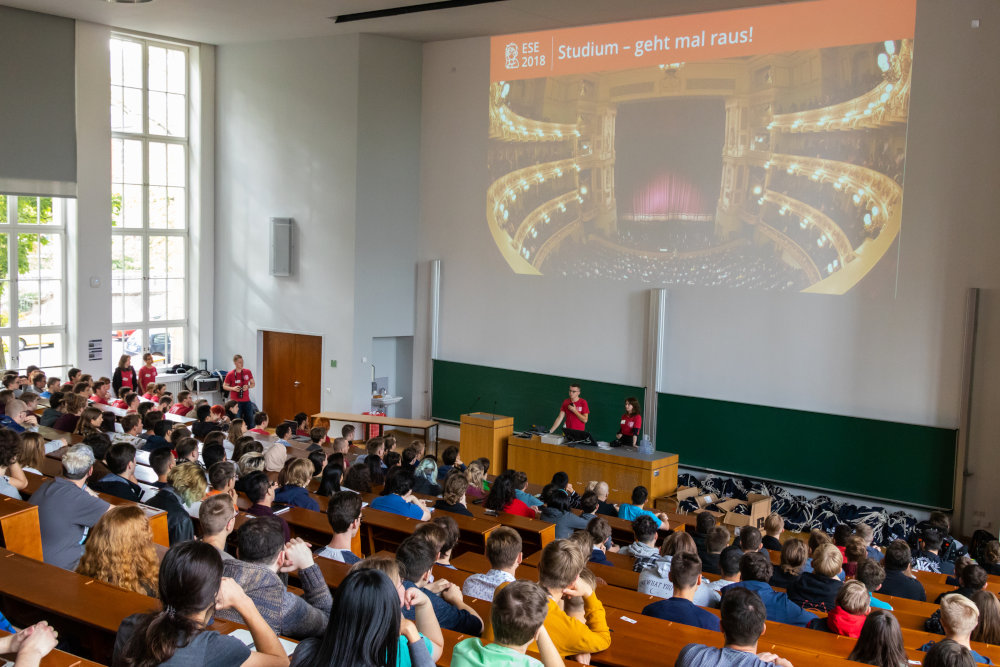
\includegraphics[width=.93\linewidth]{img/begruessung1.jpg}

\checkbox{Emeal card}
The Mensakarte allows you to pay cashless in the different refectories of the university.
You can get it during the ESE or in the refectories themselves for a deposit of 5\euro\ and by presenting the Emeal certificate, which you will find on your Semesterbogen.


\checkbox{WIFI}
You can access the internet with your devices both on campus and in the faculty premises. 
The network is called \textit{eduroam} and offers you secure internet access not only at the TU Dresden but also at many other universities worldwide. 
You get access with your ZIH login, here in the form 
   \textit{vona123a@tu-dresden.de}, 
and your password. For mobile devices like your smartphone 
\href{https://tu-dresden.de/zih/dienste/service-katalog/arbeitsumgebung/zugang_datennetz/wlan-eduroam}{%
ZIH recommends the setup via eduroam CAT}. 

\checkbox{Programming courses}
Especially for those without programming experience, the programming courses offered in the winter semester are highly recommended. 
Especially the C, Python and Java courses are very helpful to get through the first semesters. 
The courses usually take place during the week.
For details, refer to \href{mailto:programmierung@ifsr.de}{programmierung@ifsr.de} and keep an eye on the news on the \href{https://www.ifsr.de}{FSR page}.
You can also use the LinkedIn Learning courses that are accessible \href{https://www.slub-dresden.de}{through the SLUB}.

\label{sec:sprache}
\checkbox{(optional) Language courses}
TU Dresden offers language courses for English and many other languages. 
Enrollment for the language courses will be unlocked during the first two weeks of your studies, depending on the course. Check the 
\href{https://lskonline.tu-dresden.de/}{LSK pages} 
early to find out when this is. Most courses fill up very quickly.

\label{sec:sport}
\checkbox{(optional) Sports courses}
As with the language courses, it's first come, first served\ldots{} 
You can check the offer at the 
\href{https://tu-dresden.de/usz}{Universitätssportzentrum (USZ)}.
Once you have decided on a course and registered for it, all you have to do is print out the registration certificate and transfer the fee to the USZ bank account within three days.

\checkbox{Documents relevant to your studies}
The \href{https://tu-dresden.de/ing/informatik/studium/lehre}{Vorlesungsverzeichnis} and 
\href{https://tu-dresden.de/ing/informatik/studium/studienangebot}{the Prüfungs- und Studienordnung} can be found on the pages of the faculty.
Printed regulations are available at the FSR, but are also distributed during the seminar group meetings.
All important information about the individual lectures can be found on the respective pages of the institutes on the net.
The professors will tell you everything in the first lectures. 
Otherwise, a look at the \href{FSR page}{https://www.ifsr.de} might help you.

% TODO Wohnsitznachweis nach wie vor benötigt?
% (https://www.slub-dresden.de/service/benutzungsordnung/)
\checkbox{Library card}
You can get your library card at the counter of the SLUB (Zellescher Weg 18) after registering online and presenting your proof of residence, i.e. your identity card after you have changed 
\href{https://www.slub-dresden.de/besuchen/nutzerin-der-slub-werden}{your registration}.
Registration and borrowing of media is free of charge -- provided that you do not exceed the loan periods ;).

\checkbox{(optional) Visit FSR meetings}
\hyperlink{sec:fachschaftsrat}{Here}
 you can find more information about the FSR.

\checkbox{Fachschaftsrat elections}
Vote for your student representatives in the FSR Computer Science. Elections are held at the end of the year. 
Go vote! And even better: Get elected!


\checkbox{Exam enrollment}
From the beginning of next year you can register for exams in \href{https://jexam.inf.tu-dresden.de/}{jExam}.
The date will be announced on the page of the Prüfungsamt.
Register in time, otherwise you will not be able to take the exam.
Enroll in the exams of the subjects you have attended. Note that the first exam in math is already at the beginning of December. Good luck!

\checkbox{Re-registration for the summer semester}
From mid-January 2022 you can transfer the semester fee for the next semester.
You can find the exact amount and dates online \href{https://tu-dresden.de/imma/rueckmeldung}{here}.
Take care of it in time, otherwise you will be automatically exmatriculated!

\end{itemize}


\begin{figure}[h!]
\centering
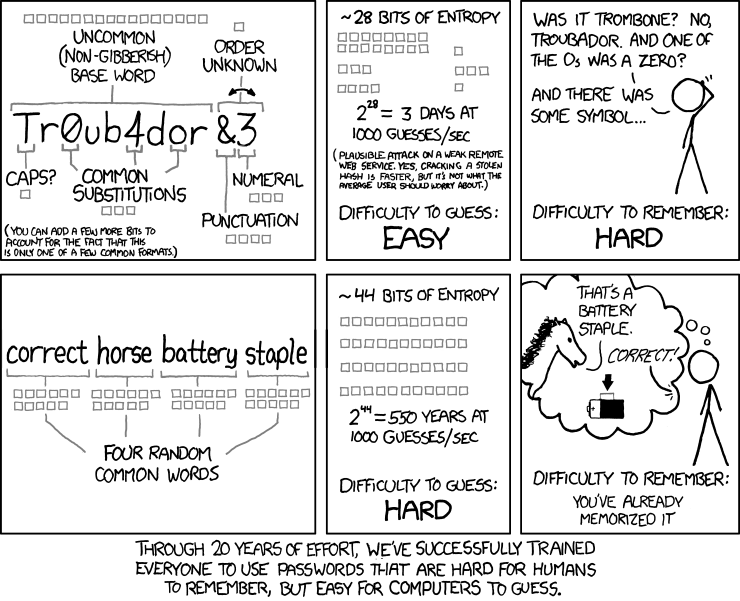
\includegraphics[width=.8\linewidth,keepaspectratio]{img/xkcd/password_strength.png}
\caption*{{\small
    \foreignlanguage{english}{
      \textit{To anyone who understands information theory and security and is in an infuriating argument with someone who does not (possibly involving mixed case), I sincerely apologize.\\\hspace*{1mm}\hfill(https://xkcd.com/936)}
    }
%     \foreignlanguage{english}{
%       \textit{\enquote*{Are you stealing those LCDs?} \enquote*{Yeah, but I'm doing it while my code compiles.}\\\hspace*{1mm}\hfill(https://xkcd.com/303)}
%     }
  }
}
\end{figure}

\chapter{Press F1 For Help}

\textit{Seminar Groups / Fachschaftsrat / Studierendenrat / Student Advisory Service / Studentenwerk 
/ Dean of Studies / Studying with Disabilities and Chronic Illness / Examination Office}


Should difficulties or questions arise at any time during your studies, don't be afraid to ask for help in time.
The principle applies: It is better to ask once too often than once too little, because, as we all know, asking costs nothing.
And let's be honest, many people before and after you will have faced and still face similar problems.
Fortunately, there are numerous ways to clarify questions and get help.
The respective lecturers and tutors are always happy to answer technical questions.
Do not hesitate for long and raise your arm, you will see that many of your fellow students will be grateful to you.
Because even if everyone around you is nodding thoughtfully while a complicated differential equation is being solved at the front of the blackboard -- the truth is that most of them, just like you, have no idea.
Are you still a bit shy at the beginning? Then remember your question and go to the lecturer before or after the lecture.

With time, you will certainly get to know fellow students from older semesters whom you can ask for help.
This applies not only to questions about the content of a lecture, but also to the course of study.
How does the crediting of this module work? When can I register for exams? Where do I have to report if I was sick during an exam?
If in doubt, contact the student council!
There you will get a confidential and usually quick answer to your question or at least the contact who can give it to you.

\section*{What to do with my questions?}
\begin{enumerate}
\item Ask your fellow students.
\item Get advice from your seminar group mentor.
\item If neither of these help, please contact the FSR. You can do this in person or by e-mail.
\end{enumerate}


\label{sec:seminargruppen}
\section*{Seminar groups}
To help you find your way around quickly at the beginning of your studies, you will be assigned to a seminar group together with other students for the first semester. You will share a common timetable. In the tutorials you will see familiar faces again and again, with whom you can form study groups. Often new friendships are formed. Your seminar group mentor is always available as a direct contact person for questions or problems. In the course of the first semester, there are several meetings where important information about the course and organization of the studies is conveyed. Therefore, you should not miss these meetings.

\label{sec:fachschaftsrat}
\section*{Student Representative Council (FSR)}


\includegraphics{img/fsr_logo.svg}

The Student Representative Council is your student representative at the faculty level.
It is elected annually and currently consists of 18 members of the Fachschaft Informatik, which you are a part of. 
The FSR office is located on the first floor in room APB/E017.
To get in touch, you can also just write an email to 
\href{mailto:fsr@ifsr.de}{fsr@ifsr.de}.

\subsection*{What can we do for you?} 

The FSR is the first point of contact for you if you have problems or questions about your studies.
It offers many useful tips and assistance, such as exam collections \url{https://ftp.ifsr.de/klausuren},
protocols of oral exams \url{https://ftp.ifsr.de/komplexpruef/} 
and consulting services, which you are welcome to make use of at any time.

In addition to supporting you in your studies, the FSR also tries to make your life beyond the university a bit more pleasant by offering social and cultural activities.
For example, the FSR usually organizes game nights with board, card and digital games once a month in the faculty.
It co-organizes Christmas parties, barbecues, hikes, sports tournaments and much more.
Last but not least, it plans the ESE together with many helpers and has created this booklet for you.

The FSR is also a central component of student participation in university committees, boards and commissions. There, for example, it has a direct influence on the revision of study regulations and the appointment of professors at our faculty. It helps to control and improve the quality of teaching, for example by evaluating lectures.

The FSR office offers the possibility to print a small number of pages. In addition, it offers various equipment and materials for rental
\url{https://www.ifsr.de/service/geraete-ausleihen}.
Among other things, you can borrow various Raspberry Pi, an Oculus Rift and Lego Mindstorms robots. 
Just drop by and bring your ID with you the first time so that you can be issued a loan certificate right away.

\subsection*{How can you get involved?} 

In many areas, the university is managed democratically from the bottom up.
This democracy thrives on participation and on people who implement ideas, projects and visions.
This has worked successfully for many decades.
To keep it that way, the FSR, just like many other bodies and groups at the university, needs active, committed, motivated members and supporters at all times.

\subsection*{Student representation is what you make of it}


\includegraphics{img/f1_neu.png}

Even if you don't want to stand for election yourself, you can do something for your student council.
The first step is to vote. This costs very little time and is important to legitimize the FSR and to give it support for the representation of student interests.
And how about, for example, participating in the ESE yourself next year?
Or maybe teach a programming course?
We are always looking for organizational talent and contributors for individual events like the sports tournaments or the Lange Nacht der Wissenschaften.

So if you don't want to be officially elected for the whole year, you can always help and contribute.
There are enough tasks or ideas and you are welcome to bring your own.

Normally, the FSR meets every Monday at 18:45 in the large council room (APB/1004) to discuss various topics, such as committee work, upcoming events and demonstrations, but also problems and developments at the faculty and university. You are cordially invited and can just drop by, because the meetings are usually open to the public. On the website of the FSR \url{https://www.ifsr.de}  you can find the minutes of the meetings and a lot of other useful information. Due to the current situation regarding Covid-19, meetings are also held online via Big Blue Button  \url{https://www.ifsr.de/events/fsr-sitzung}.

\section{Student Council (StuRa)}\label{sec:stura}

The Student Council, often known as the Allgemeiner Studierendenausschluss (AStA) and the Studierendenparlament (StuPa) in other German federal states, is the body that is superior to the student councils and represents the interests of all students at the TU Dresden.

However, it also offers a range of services, including: 


\begin{itemize}
\item BAföG and social counseling
\item legal advice
\item Counseling for foreign students
\item Advice for students with children
\item Advice on applications and funding opportunities
\item Sale of tickets for various cultural events
\end{itemize}

Detailed information can be found on the StuRa website \url{https://www.stura.tu-dresden.de}.

% Wird der gedruckte Spirex eigentlich noch aktualisiert? Die PDF ist von 2014/15 :/

\section{Student counseling}

Sometimes studying does not go smoothly. Individual students have orientation difficulties or problems coping with the requirements, especially at the beginning of their studies.
The Student Advisory Service supports you with information in all phases of your studies. The counseling covers, for example, questions about exams and exam preparation, specialization options, changing majors, or questions about scheduling.
The TU Dresden offers a general, inter-faculty student advisory service \url{https://tu-dresden.de/studium/im-studium/beratung-und-service/zentrale-studienberatung} 
which can help you, for example, with doubts about the choice of study program, exam anxiety or similar concerns.
For all questions and problems specific to a study program, our faculty has its own counseling services with contacts among students and non-students
\url{https://tu-dresden.de/ing/informatik/studium/beratung}.

\minisec{Studierendenwerk (StuWe)}
\label{sec:stuwe}
The Studierendenwerk not only runs the dormitories and provides good and inexpensive meals in the dining halls and cafeterias, but also offers extensive support and assistance for students. These include:
\begin{itemize}
\item Legal and social counseling
\item Psychosocial counseling
\item Processing of BAföG applications
\item Assistance for students with disabilities
\item Pregnancy and childcare during studies
\end{itemize}

Further information about the tasks and offers of the StuWe can be found on the internet 
\url{https://www.studentenwerk-dresden.de/}.


\minisec{Dean of Studies and Student Representative}
There are many different offices in the Faculty. The highest and most important is the role of the dean of the faculty and his deputy, the vice dean. However, for teaching and thus your studies, the so-called Dean of Studies is of great importance. He is responsible for the affairs of teaching in the faculty, mediates between students and teachers and helps with problems with the study in general.

\pagebreak
\textbf{Dean of Studies for German-language degree programs}\\
Prof. Dr. rer. nat. habil. Gerhard Weber \\
Office: APB/1055 \\
Phone: (0351) 463-38477 \\
E-mail: gerhard.weber@tu-dresden.de

\textbf{Dean of Studies for English-language degree programs}\\
Prof. Dr. Christof Fetzer \\
Office: APB/3104 \\
Phone: (0351) 463-39709 \\
E-Mail: christof.fetzer@tu-dresden.de

\textbf{Representative for the teaching degree programs}\\
Prof. Dr. rer. nat. Nadine Bergner \\
Office: APB/2096 \\
Phone: (0351) 463-38306 \\
E-Mail: nadine.bergner@tu-dresden.de

\minisec{Study with Disability and Chronic Illness}

At the TU Dresden we are always working on a barrier-free design of the studies as well as the study environment. If you have a health impairment, special questions and issues around your studies often arise. Numerous support and counseling services are available to help you participate in your studies in a way that is appropriate for you~\link{https://tu-dresden.de/studium/rund-ums-studium/studieren-mit-beeintraechtigung}.


\refstepcounter{dummy}\label{sec:pruefungsamt}
\minisec{Prüfungsamt (PA)}
The Prüfungsamt is responsible for registering students for examinations, announcing results, managing examination files and other matters relating to examinations. You will find a lot of information, forms and frequently asked questions on the pages of the Prüfungsamt~\link{https://tu-dresden.de/ing/informatik/studium/pruefungsorganisation}. Examination schedules and registration deadlines are also announced there. During the open office hours, you can also submit your applications and questions without an appointment in room APB/3039.

\textbf{Contact}

Phone: (0351) 463-38230

E-Mail: \href{mailto:pruefungsamt.inf@tu-dresden.de}{pruefungsamt.inf@tu-dresden.de}


\chapter{The Faculty of Computer Science}

The \emph{Andreas-Pfitzmann-Bau} (APB in short) houses the Faculty of Computer Science and will therefore be your second home for the next few years. As the number of semesters increases, you will be shooed around the campus less and less and more events will take place here. But what does this building actually have to offer besides a lot of green paint and the sculpture in the foyer?

\begin{figure}[h!]
    \centering
    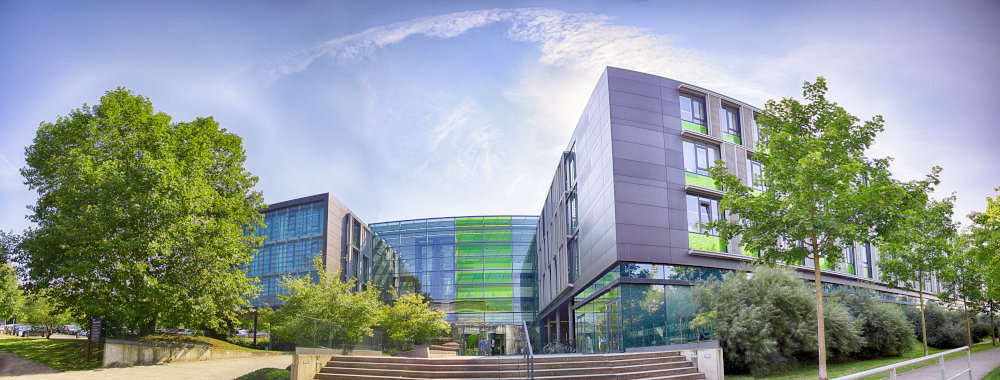
\includegraphics[width=\linewidth]{img/panorama_fakultaet1.jpg}
    \caption*{\small \textit{Der Andreas-Pfitzmann-Bau von vorn -- Foto: Lucas Vogel}}
\end{figure}

One difference between this building and the others on campus is that it is open around the clock. Even if the doors are locked at night, the security service will be happy to open the door for you upon presentation of your student ID and, if you wish, unlock one of the seminar rooms on the first floor.

There is plenty of space to sit in the corridors of all floors, for example to prepare for upcoming exams with your study groups. Furthermore, there are several PC pools, some of which are equipped with special software, but which are only open during the day.

\label{sec:apb}
We also have a large outdoor area. Due to a construction project, however, the pond and the sunbathing lawn are unfortunately not very inviting at the moment.

\begin{figure}[t]
    \centering
    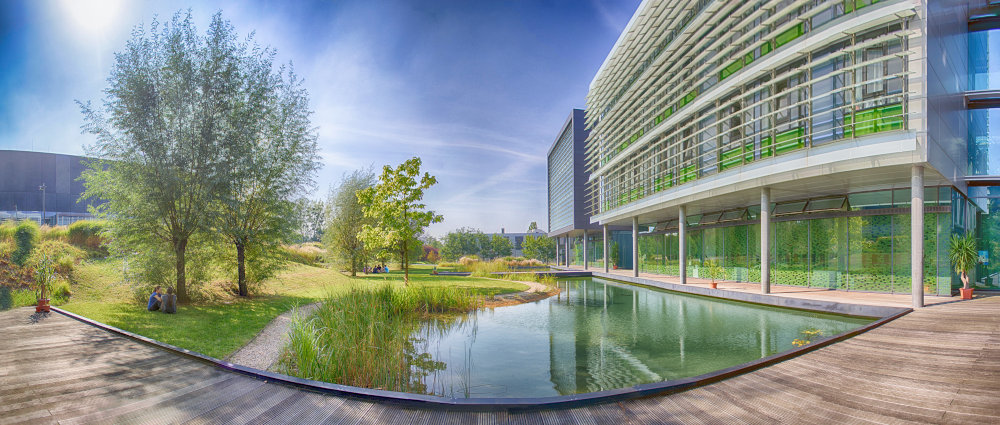
\includegraphics[width=\linewidth]{img/panorama_teich1.jpg}
    \caption*{\small \textit{Der Außenbereich bevor die Bagger kamen -- Foto: Lucas Vogel}}
\end{figure}

This idyll had to give way to a construction site for the time being, as a new building is being erected behind the APB. In addition to many members of the faculty, also your student representatives campaigned for the preservation of the outdoor area with the \href{https://savethetei.ch/}{\#SaveTheTeich campaign}.
The great commitment and tough negotiations paid off: the pond is to be largely restored after the end of construction. To compensate for the lost space on the current slope, above-average funds have now been earmarked for equipping the remaining areas with seats and sufficient greenery. We all hope that the outdoor area will soon shine in new splendor, invite you to take a break and serve as a cozy meeting place again.

From the APB you can see the Rechenzentrum (\enquote{Lehmann-Zentrum}). Maybe you'll get the chance to take part in one of the guided tours through the Rechenzentrum that are offered at various events.

By the way, the building takes its name from Andreas Pfitzmann, one of our professors who died in 2010. For many years, he headed the Chair of Data Protection and Data Security, where he was instrumental in researching ways to make data anonymous, thus enabling many people in countries with censorship and state surveillance to freely access the Internet. In 2009, he also became dean of our faculty. In the foyer you will find a plaque commemorating him and his life's work.

\pagebreak

\minisec{\textbf{ascii} – The café in the faculty}

Since 2007 \ascii{} is located in the building of the Faculty of Computer Science. It is a café run by students who spend a few hours of their free time behind the counter.

The \ascii{} has everything a real café needs: coffee, tea, a variable assortment of savory as well as sweet drinks and of course caffeinated cold drinks. In addition, \ascii{} is one of the few places on campus where you can get Club Mate as well as Kolle Mate and Premium Cola.

\begin{figure}[h!]
    \centering
    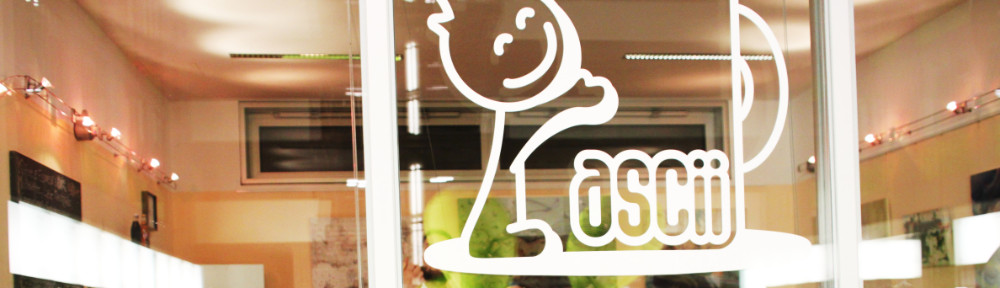
\includegraphics[width=\linewidth]{img/ascii.jpg}
\end{figure}

The \ascii{} is run by a student association and has been a central contact point at the faculty since its founding. Students and employees meet here to spend their breaks, work or simply replenish their caffeine supply. On the comfortable sofas you can let time pass by, work together on projects, learn, program or just chat with fellow students.

If you now feel like visiting ascii or even joining as a member yourself, just drop by and say hello!

For more information, visit~\link{https://www.ascii-dresden.de/}.

\begin{awesomeblock}[ese_bg_color]{2pt}{\faCalendar*[regular]}{ese_bg_color}
    \textbf{Opening hours during the semester}

    Monday to Thursday: 9 a.m. to 5 p.m.

    Fridays: 9 a.m. to 3 p.m.
\end{awesomeblock}

\chapter{The Campus++}

Although some may wish it, not all of your studies will take place in one building. Instead, there are a few key buildings that will play a role in your day-to-day studies.

\minisec{HSZ}
Especially the basic lectures do not take place in the APB, but in the Hörsaalzentrum (\emph{HSZ}). In this building, which is very monotonous compared to the APB, you will experience many of your lectures and accumulate one or the other kilometer while commuting between the APB and the HSZ. The HSZ has four lecture halls, including the Audimax, the largest lecture hall at the university and the largest auditorium in Saxony. In addition, there are some seminar rooms, in which tutorials can take place. Behind the \enquote{central cube} is the beautiful meadow of the HSZ\@. You can not only relax on it. Parties and fairs also take place there regularly.
In addition, the Grillcube with burgers and the like is there for small appetites, as is the Pasta-Mobile with fresh pasta.

\minisec{Willersbau}
The Willersbau~\link{https://navigator.tu-dresden.de/etplan/wil/00} is the mathematics building at the TU Dresden. This is where some of your math tutorials take place. The Willersbau is in the immediate vicinity of the HSZ and the Trefftzbau, which houses the math lecture hall.

\minisec{Trefftzbau}
This~\link{https://navigator.tu-dresden.de/etplan/tre/00} is usually where parts of your math lecture take place. Since the building is being renovated and exceptions prove the rules, no lectures are held there at the moment due to the renovation. In front of the Trefftzbau is the Trefftzwiese, which is a wonderful place to relax after a lecture, especially in the summer.

\begin{figure}[b!]
    \centering
    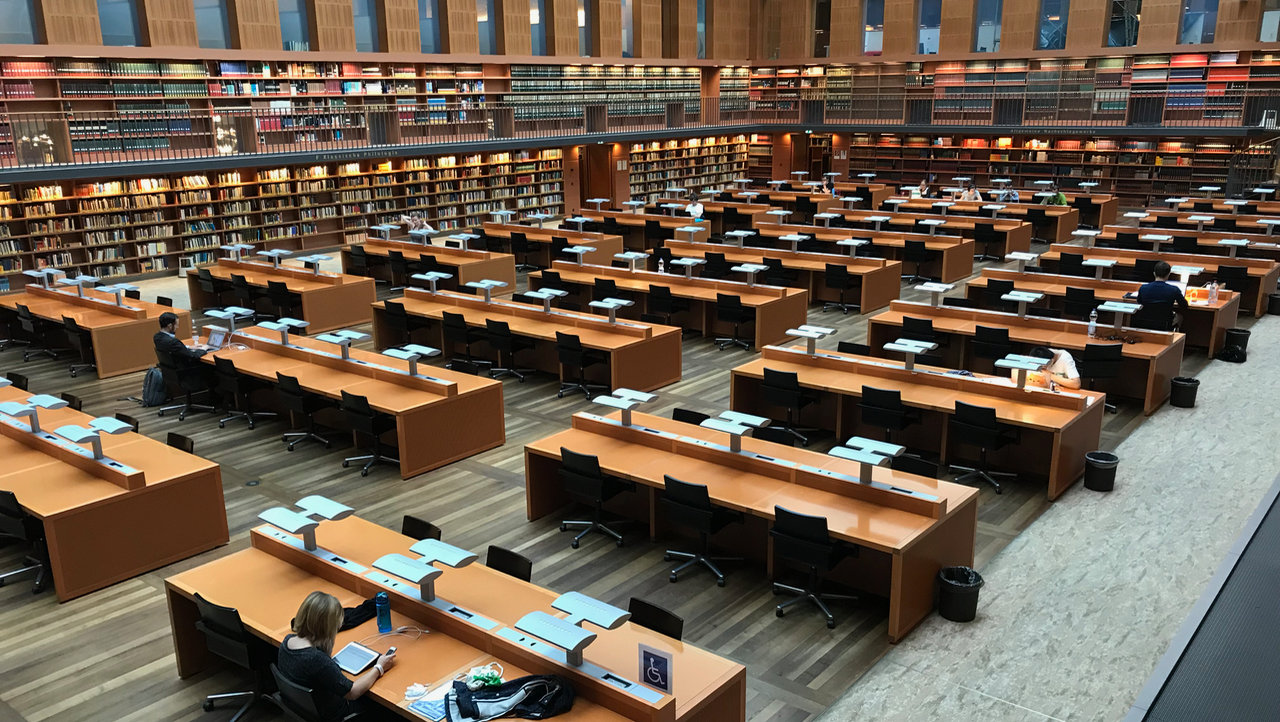
\includegraphics[width=\linewidth]{img/slub-lesesaal.jpg}
\end{figure}

\minisec{SLUB}
\label{sec:slub}
The Sächsische Landesbibliothek - Staats- und Universitätsbibliothek Dresden, \emph{SLUB}~\link{https://slub-dresden.de} in short, is what is simply called Bib at other universities.
With a selection of over 12 million holdings consisting of books, magazines, films, etc., it is one of the largest (university) libraries in Germany. In addition to haptic reading material, the SLUB also offers an extensive selection of online resources that you can download free of charge as a student. Many of the books that are recommended to you in basic lectures are in stock at the SLUB in large quantities. So a trip to the textbook department can save you a lot of unnecessary expenses. Across from the main building is the DrePunct, a branch of the SLUB where most computer science textbooks are stored. If you are looking for a specific book, it is advisable to check the SLUB website to find out where the book is located. This will save you most of the search and will show you whether the book you are looking for is currently available.\newline
But even for notorious non-readers, the SLUB is a popular place to stay because of the many workstations. If you want to study together with others, there is a spacious entrance area with group tables. In addition, private group rooms can be reserved. If you prefer to study alone, there are of course enough quiet places for you in the SLUB\@. The quietest workplaces can be found in the central reading room in the second basement, which can also be seen in the picture below. A nice café, where you can pay by Mensa card, completes the whole experience.

\newpage
\minisec{Seminargebäude}
The language courses of the LSK take place in the Seminargebäude, recognizable by its particularly beautiful facade. For those who want to go beyond a simple language course, additional seminars on the culture and politics of selected countries and regions are offered. More information can be found on the website of the LSK~\link{https://tu-dresden.de/gsw/slk/lsk}.
The building is right next to the SLUB.

\minisec{refectories}
Fortunately, if you don't want to spend your studies ordering pizza, you don't have to, because the Studierendenwerk operates a network of 18 refectories.
No matter in which building of the university you are, you will find a refectory or at least a café nearby.
The daily menu of all refectories can be found on the Studierendenwerk pages ~\link{https://www.studentenwerk-dresden.de/mensen/speiseplan/}.

The largest of the refectories, the Alte Mensa, is fortunately located directly between the APB and the HSZ\@. Here you will find a variety of daily changing main dishes, salads and desserts. For friends of late breakfasts or students with disturbed sleep rhythms, the Alte Mensa offers a warm evening meal until 7 p.m. between Monday and Thursday. However, the selection becomes increasingly limited after 3 p.m. Since the refectory can hardly cope with the abundance of people at peak times, it is advisable to have meal times that do \emph{not} start directly after the end of a lecture.

If you do not like what the Alte Mensa has to offer, you are welcome to take the 10-minute walk to the Zeltschlösschen. The Zeltschlösschen is a classic refectory that is inferior to the Alte Mensa in pretty much all respects.

In five minutes you can also reach the Bio-Mensa U-Boot. The ingredients used in this refectory are organic and locally produced. The meat used in the Mensa U-Boot comes directly from the west of Dresden, which increases the price of the meals considerably. However, the prices of the meatless alternatives should not differ much from those of other refectories.

You can also escape cooking on weekends, because the Mensa Siedepunkt is also open on Saturdays and Sundays. Especially after a productive study session at the SLUB, it is very easy to get there by simply changing sides of the street.

\paragraph{FSR Insider Tip:}
Without a doubt, the most popular cafeteria on campus, if you believe the statements of Dresden FSR students, is Firat.
This is an independent kebab store, but due to its efficient handling of above-average student crowds, it likes to be jokingly referred to as a refectory.
It only takes a 10-minute walk from the APB to get there and attracts with good quality, cozy ambience and a comparatively large selection of dishes.

\minisec{student club Count Down}


\includegraphics[width=\linewidth]{img/countdown.svg}

Dresden is considered the unofficial capital of student clubs; after all, there are 15 of them here.
The Studentenklub IZ e.V. also runs a small student club, the Count~Down, in the depths of the dormitory Güntzstraße 22.
IZ stands for Informatikzentrum (computer science center) and in fact this is the last remnant of the computer science faculty in Johannstadt, where it had its home until the mid-2000s.

In addition to a large selection of the best beers and the tastiest mate (drink) at student prices, the Count~Down offers a wide range of events. Various metal parties, the joint Erasmus country night with the ESN initiative of TU-Dresden as well as game and cocktail nights are part of the regular repertoire.
You can find out more about it here~\link{https://www.countdown-dresden.de/}.

Of course you should check out other student clubs as well~\link{https://vdsc.de/}.

Generally, the operation of the student clubs is ensured by voluntary commitment, so they are always looking for new blood and fresh ideas. Just get in touch with your favorite club if you can imagine being behind the bar or taking on other tasks.

\textbf{opening hours}

Mondays: 7 p.m. to midnight

Tuesdays: 8 p.m. to 1 a.m.

Wednesdays: 7 p.m. to midnight

occasionally on Saturdays

\chapter{Events}
\label{cha:veranstaltungen}

All events mentioned here are also advertised on social media and via posters in the faculty shortly before they actually take place. So check back regularly for detailed information on
Facebook~\link{https://www.facebook.com/iFSR.de/},
Instagram~\link{https://instagram.com/ifsrde},
Twitter~\link{https://twitter.com/ifsr} or on our
website~\link{https://www.ifsr.de}. 
In addition, we also operate a telegram channel~\link{https://t.me/ifsrde}, through which we also keep you up to date.

\minisec{Game nights}

About once a month, the FSR hosts a game night in the APB. It starts at 6:30 pm in the foyer. 
The FSR offers a wide range of games, so that a lot of games are already available. 
If you want to play something that is not there, you can also bring your own games along. Often you can quickly find people to try out a new game.

Every now and then a few people bring their notebooks and throw a small LAN party or bring their game consoles to play together with others via one of the projectors in the seminar rooms.

Nibbles and drinks will be provided, and the \ascii{} is usually open for game nights. 
If the weather cooperates, the student club \emph{Count Down}, is also on site and sells grilled food and alcoholic beverages.

So it's definitely worth stopping by and meeting new people over a mate and a fresh bratwurst or some grilled cheese!



\minisec{Stammtische}

Have you always wanted to get to know your favorite teacher a little more personally? The biannual Stammtisch offers exactly this opportunity. Here you sit down in a relaxed atmosphere with the two participating teachers in a student club and can ask all the questions that have been burning on your tongue for a long time, or perhaps not so long. These are not only technical questions, but also personal ones. The participating teachers are also looking forward to the active participation of the students!

\begin{figure}[b!]
	\centering
  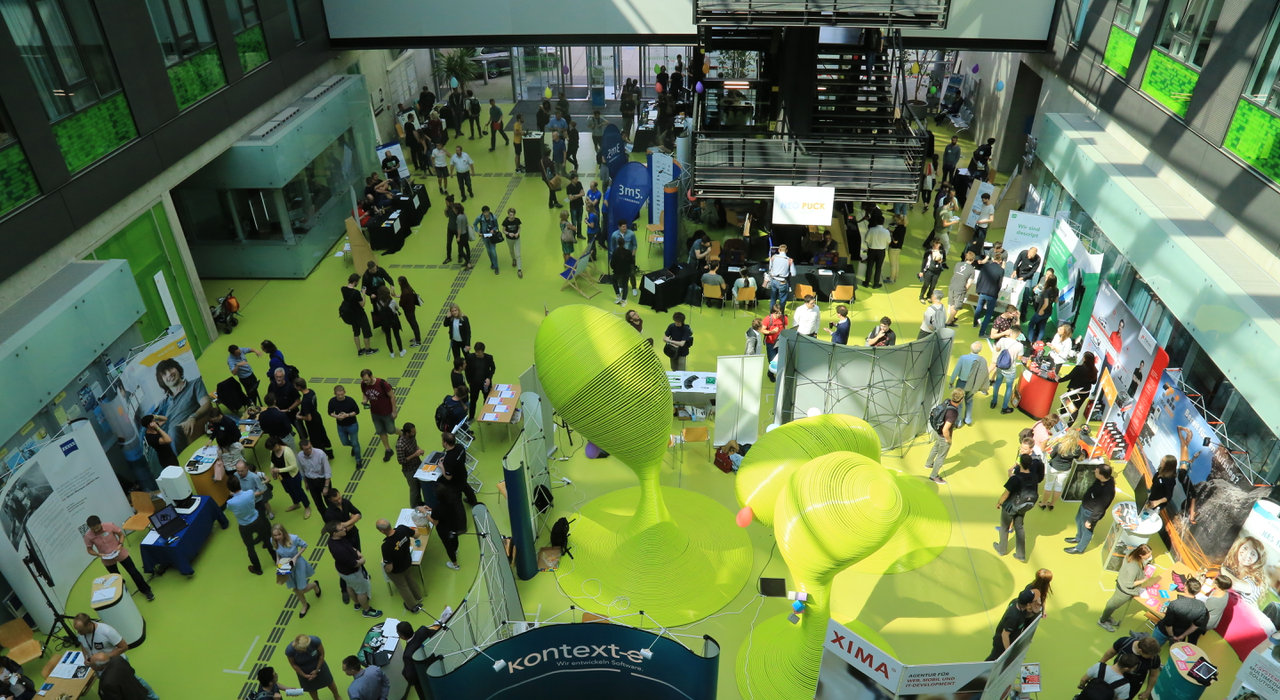
\includegraphics[width=.95\linewidth,keepaspectratio]{img/output.jpg}
  \caption*{\small \centering \textit{OUTPUT\@: Studierende stellen ihre Projekte und Firmen sich selbst vor. -- Foto: Lucas Vogel}}
\end{figure}%

\minisec{Schreibcaf\'e}

You have to write a paper, but you just can't get on with it? 
Help is usually available every Thursday at the \ascii{} Schreibcaf\'e. 
There, writing tutors from the Schreibzentrum will help you with working techniques and feedback to get ahead with your seminar paper or thesis. 
Additionally, there is almost always someone present who can help you with your \LaTeX problems over a cup of coffee.
Due to the current situation regarding Covid-19, the Schreibcaf\'e will not take place weekly and in attendance as usual. 
As soon as this is the case again, you will be informed via our social media and posters in front of the \ascii.
If you need urgent help, you can of course contact the FSR at any time.


\minisec{Dies Academicus}

The Dies Academicus is a lecture-free day where you can get to know other departments and university groups. 
There are workshops, cultural events and much more to get to know the diversity of the campus.

\minisec{Lange Nacht der Wissenschaften}

During the Lange Nacht der Wissenschaften, the university and other research institutions open their doors and prepare an evening program in which they convey what they are working on. Here you can have a look at what is happening in the other areas of the university. Often, the ZIH also offers tours of the thoroughly impressive Rechenzentrum.

\minisec{OUTPUT.DD}

The 
\href{https://output-dd.de}{OUTPUT.DD}
takes place once a year. The stated goal of this event is to present the results of teaching and research to the general public. For this purpose some big companies come to our beautiful faculty and present themselves in the foyer. For you as a student of our faculty this offers \emph{the} chance to familiarize yourself with the companies of the region and to get into conversation with them in an informal setting. This can be a good stepping stone for possible internships or working student jobs. Furthermore, there are often small raffles and contests with prizes for visitors. A visit to OUTPUT is therefore highly recommended. It is worth it!

\minisec{ESE}

The Erstsemestereinführung (ESE) takes place every year at the beginning of October to welcome the new students of our faculty and to introduce them to their studies. 
It is organized by the FSR, which usually starts planning the next ESE shortly after the current one has ended. As you can imagine, this is quite a lot of work, at least if there is no one to help.

This is where you come in. Did you think your ESE was great and want to make sure that all other first-year students have a great ESE as well? Or did you find your ESE absolutely horrible and have a thousand ideas how to make it better? Then get in touch with us at the FSR office and help us with the next iteration of the ESE! We are happy about any help. :)

% \begin{figure}[b!]
%   \centering
%   \includegraphics[width=\linewidth]{img/output_pond}
%   \caption*{\small \centering \textit{Zur OUTPUT wird der Teich zur Lounge -- mit Musik, Freibier und frischem Essen vom Grill. Foto:~Lucas~Vogel}}
% \end{figure}



\chapter{Everyday life at university}

When you start your studies, you will be faced with new tasks and challenges that need to be mastered. The following pages will give you an impression of how your studies are structured and how learning at the university works.
But be sure to also read your Studienordnung~\link{https://www.verw.tu-dresden.de/AmtBek/PDF-Dateien/2016-06/11soBA24.04.2016.pdf}
and Prüfungsordnung~\link{https://www.verw.tu-dresden.de/AmtBek/PDF-Dateien/2016-06/11poBA24.04.2016.pdf}.

\minisec{Modules}
When you start your studies, you will be faced with new tasks and challenges that need to be mastered. The following pages will give you an impression of how your studies are structured and how learning at the university works. But be sure to also read your study regulations 58 and examination regulations 59.
Modules
In the course of your studies you have to successfully complete numerous so-called modules. A module can contain several courses. These can be lectures, tutorials, internships or seminars. Many modules consist of only one lecture and one tutorial. You complete a module by passing the module exam. A module examination can consist of one or more examinations (e.g. written examinations). Sometimes a preliminary examination must be passed before you are allowed to take part in the real exam. For the individual modules, Appendix 2 of the Studienordnung (Modulbeschreibung) specifies exactly which examinations must be taken.
Each module has a specified number of credit points (LP, often also called credits or ECTS points). One LP corresponds to a workload of 30 hours. If a module is worth 5 LP, this means that 150 hours of work are required over the course of the semester. This workload consists of attendance time (time you actually spend in lectures/tutorials at the university), time for preparation and follow-up of the courses (self-study), exam preparation and the exam itself. The LP for a module will be recognized after passing the module exam.

\minisec{Timetable}

At the university there is a so-called course schedule, which is published shortly before the beginning of each semester. You can find this list of courses, which is already sorted by semester, online on the Faculty's page~\link{https://www.inf.tu-dresden.de/}.
Your task is to create your own timetable from this list. For the beginning you will get ready-made timetables from us, from which you can then simply choose a timetable to enroll in jExam. Don't worry, we will do it together with you at ESE.

\pagebreak

While lectures generally have a fixed date, tutorials are flexible.
Simply register for the tutorials of your choice at jExam~\link{https://jexam.inf.tu-dresden.de/}.
However, if you find out later that your tutor has the qualities of a sleeping pill or that the tutorial is too full for you, do not hesitate to change it.

If you look at the available courses, you will come across the abbreviation SWS. SWS stands for Semesterwochenstunden and indicates the time required for a course. SWS is only a statement about the attendance time at the university. The time for preparation and wrap-up is not taken into account. 1 SWS means that the course is taught for an average of 45 minutes per week during the lecture period. A course with 4 SWS is taught for 3 hours per week. A teaching unit at the university lasts 90 minutes and is called a Doppelstunden (DS). A course with 4 SWS is therefore taught 2 times a week. It is a bit more complicated if a course is actually only 1 SWS. In this case, the course only takes place every 14 days and you have to check exactly whether the course takes place in even or odd calendar weeks. In the timetable you will then find the designations \enquote{1st\ week} or \enquote{2nd\ week}. These have nothing to do with the weeks relative to the beginning of the semester! \enquote{1st\ week} means that the course takes place in every odd calendar week and \enquote{2nd\ week} stands for even calendar weeks.
\begin{figure}
	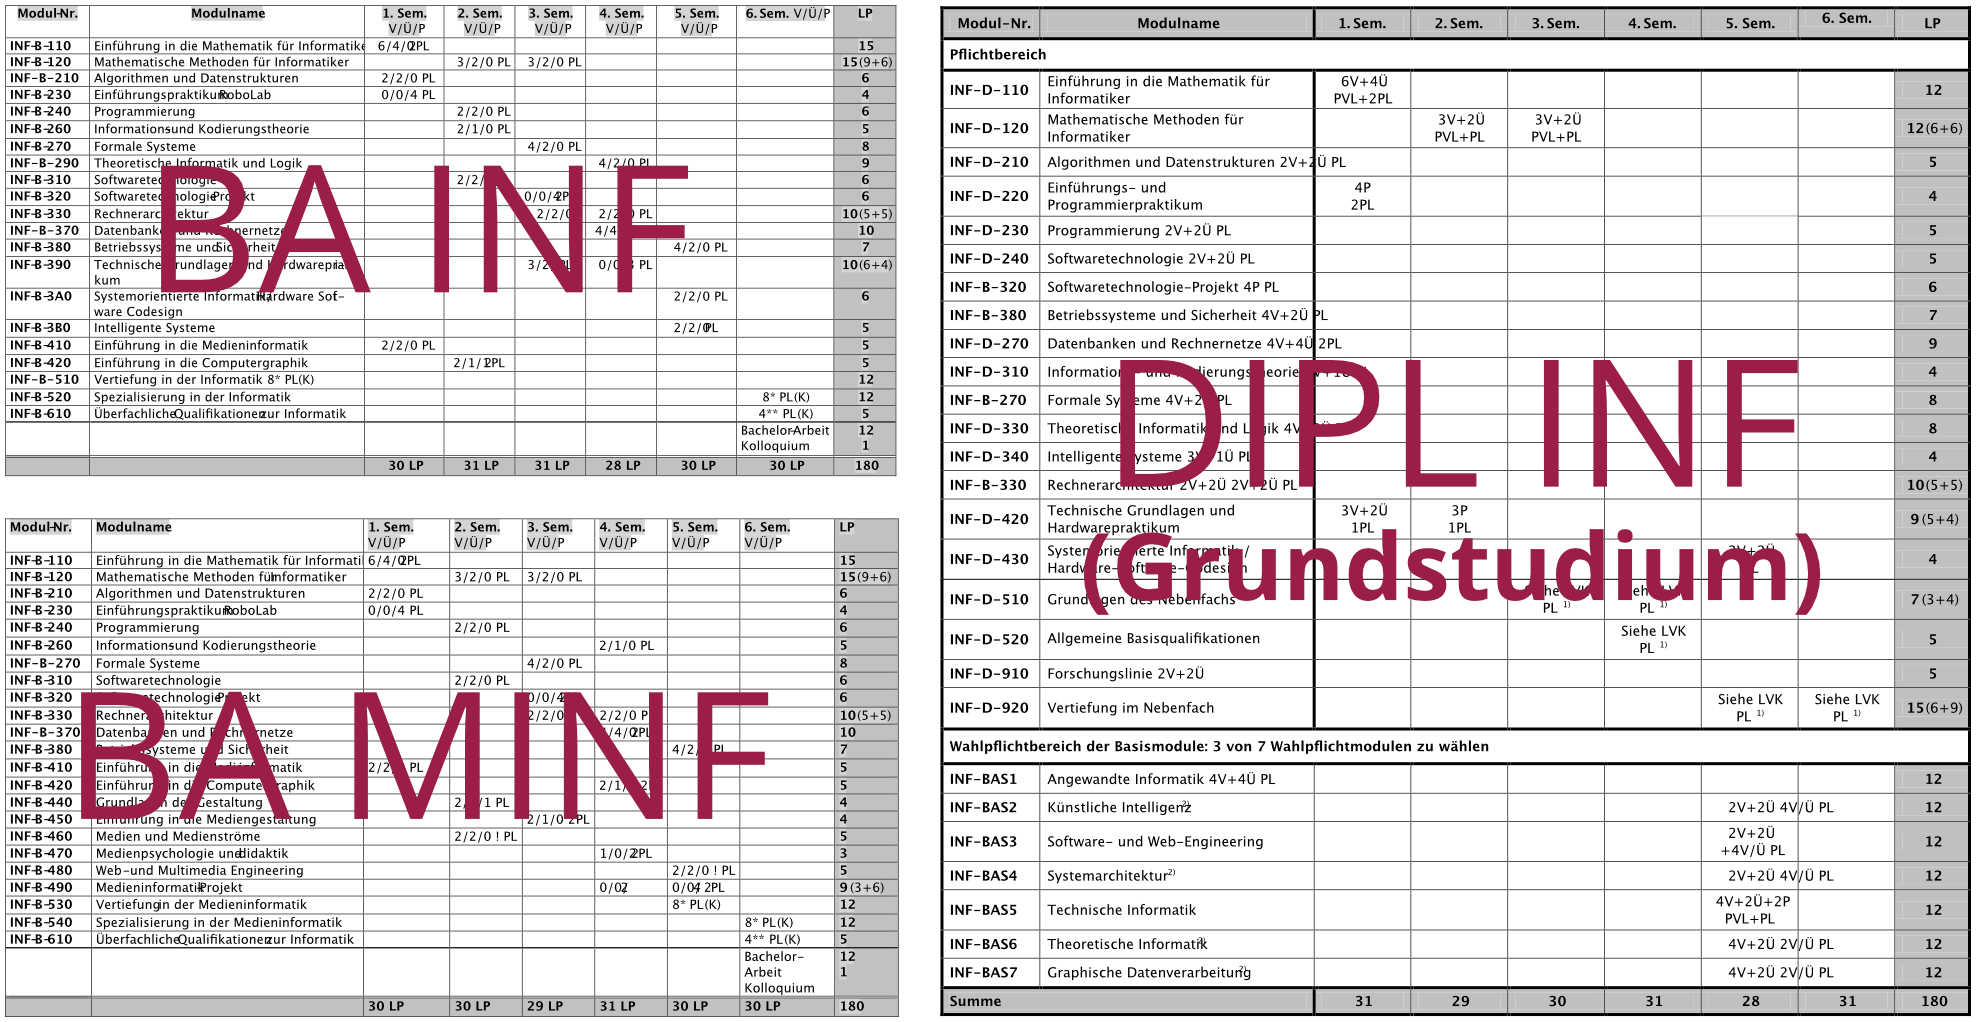
\includegraphics[width=\textwidth]{img/alle_studienablaufplaene.png}
	\caption*{\small \textit{Die Studienablaufpläne aller Studiengänge findest du in groß unter}~\link{https://tu-dresden.de/ing/informatik/studium/studienangebot}.}
\end{figure}

\minisec{Lecture}

In the lecture, the material is taught that will ultimately be asked in the exam. It is therefore advisable to actively follow the lecture and, if necessary, to prepare and follow up on it. It is not advisable to catch up on all the material before the exam, as the amount of material is usually very large and it would mean unnecessarily more stress during the exam phase.
\\
Especially at the beginning of your studies, the number of people attending a lecture is in the triple digits. Usually you will get used to this quickly. However, the more people there are in a lecture, the more likely it is that someone will not be able to keep up at some point in the lecture. This can happen to anyone. So if you are that someone, don't be shy about asking the lecturer a question. Active participation in the lecture is always appreciated by the lecturers. And yes, even if it is a question of understanding. Your fellow students who had the same question but didn't have the courage to ask will be happy. \\
Which lecture you should attend in which semester can be found in the respective study plan of your study program
(Bachelor Informatik~\link{https://www.verw.tu-dresden.de/AmtBek/PDF-Dateien/2016-06/11soBA24.04.2016.pdf}, Bachelor Medieninformatik~\link{https://www.verw.tu-dresden.de/AmtBek/PDF-Dateien/2016-06/11soBAMI24.04.2016.pdf}, Diplom Informatik~\link{https://tu-dresden.de/die_tu_dresden/fakultaeten/fakultaet_informatik/studium/dateien/studien_und_pruefungsordnungen/dipl_inf_so_app1_de.pdf}) or in the course catalog on the page of the faculty~\link{https://tu-dresden.de/ing/informatik/studium/lehre}. 


\minisec{Tutorial}

Tutorials are offered for almost all lectures and serve to work on tasks related to the current lecture material. Exams are often based on the tutorials, so you should visit the tutorials regularly. The tutorials are usually held by students from higher semesters or by faculty members, not by the professor. This also has the advantage that you understand many things better when they are explained to you by someone else. You can find the current tutorials on the page of the respective lecturer, often under the headings Teaching or Lehre. It is expected that you look at the exercise sheets before the tutorial in order to discuss solutions or questions.


\minisec{Internship}

The first internship awaits you during the lecture-free period of the first semester -- so don't plan your vacation too quickly! There you will prove your skills in the introductory internship \textit{Robolab}. Diploma students must also complete the Strategiespiel internship. A full internship semester is only mandatory for diploma students in the 7th semester. Of course, it is still advisable to do internships at real companies outside the faculty during the semester break. This not only increases your job chances, but also shows you whether your choice of study was really the right one.

\refstepcounter{dummy}\label{sec:pruefungen}
\minisec{Exams}
The exam period follows directly after the lecture period - probably the most stressful time in a student's life. You can find the exact exam dates for the winter semester usually around the beginning of January on the homepage of the faculty~\link{https://tu-dresden.de/ing/informatik/studium/news} or directly at the Prüfungsamt~\link{https://tu-dresden.de/ing/informatik/studium/pruefungsorganisation}.
During the semester you have the opportunity to register for the exam (within the registration period) via jExam.
here you also have the possibility to deregister up to three \emph{working} days before the exam. You can also take the exam in a later semester. Of course, this should not become the rule. For oral and other exams there is a withdrawal period of 14 days.
If you have to withdraw from the exam due to a sudden illness, you can find out on the website of the examination office which certificates you have to submit to the Prüfungsamt within which time limit ~\link{https://tu-dresden.de/ing/informatik/studium/pruefungsorganisation/pruefungen/abmelden-ruecktritt-krankheit}.
Exams are graded with grades, and all exams graded better than 5.0 are considered passed and cannot be repeated. Grades worse than 5.0 do not exist. Thus, a 5.0 is the only chance you have to fail an exam. Once you have done that, there is the possibility to repeat the exam within two semesters. After the second failed exam attempt, you only have one semester until the third one has to be taken. Only when you have failed the exam for the third time (i.e. the second retake), you will be exmatriculated. More detailed information on this topic can always be found in the Prüfungs- bzw.\ der Studienordnung, which you should definitely have a look at.
By the way, your first math exam is already waiting for you in December: the so-called Santa Claus exam.

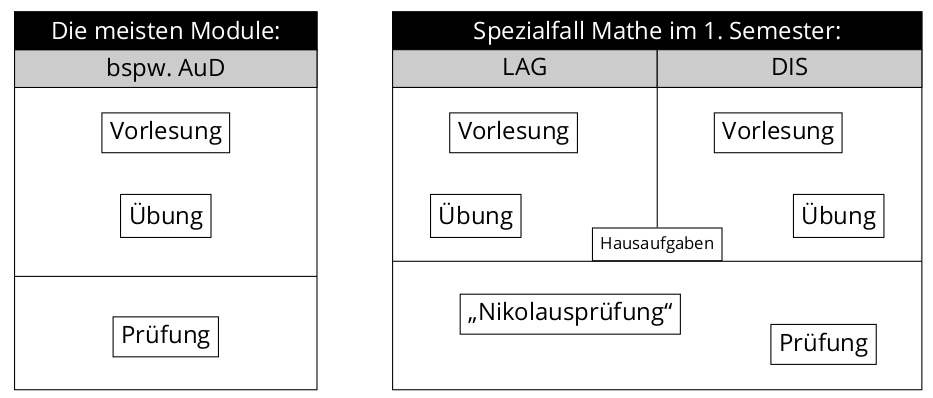
\includegraphics{img/nikolauspruefung.png}

\minisec{certificate of achievement}

For some exams, you will receive a certificate of achievement (or Schein in short) in addition to your grade. These include language courses, the research line, and in some cases minor subject examinations. You need these certificates in order to be able to have these achievements credited to you in the Prüfungsamt.

\refstepcounter{dummy}\label{sec:sprachausbildung}
\minisec{Language courses}

Courses for almost all possible (and impossible) languages are offered at the TU Dresden. For this purpose there are two centers for language education: The \enquote{Lehrzentrum Sprachen und Kulturen} (LSK) and \enquote{TUD Institute of Advanced Studies} (TUDIAS).
DThe language courses offered by the two institutions are very similar. You have a budget of Semesterwochenstunden (10 SWS in total) for various language courses, which you can spend as you wish. For your bachelor studies in (Medien-)Informatik, language courses are generally optional, but definitely recommended. For diploma students, 2 semesters of English are mandatory during the course of studies. However, if you study Bachelor Informatik and want to continue with the Master Informatik at the TU Dresden afterwards, you will have have a proof of a B2 level in English, so it might be a good idea for you to attend the corresponding language courses. The enrollment for a language course is done online~\link{https://sprachausbildung.tu-dresden.de} with your ZIH login.
As soon as the courses are activated, you should hurry, because the popular courses are usually full within a few minutes. You can find more information on~\link{https://tu-dresden.de/lsk}~and~\link{https://www.tudias.de/}.


\minisec{Writing Consultation}
The Schreibzentrum of the TU Dresden~\link{https://www.facebook.com/SchreibzentrumTUD} is a cooperative project for students and teachers of the Center for Continuing Education and the Career Service. It offers support, methods and ideas on the topic of \enquote{scientific writing}.
You can either come to the open writing consultation hour at the SCS ServicePoint of the SLUB with your writing projects of all kinds (voucher, seminar paper, thesis, etc.) or make an individual appointment by e-mail~\link{mailto:Schreibzentrum@mailbox.tu-dresden.de}.
It does not matter how far along the work is, i.e. whether you are still at the very beginning or shortly before submission. It is also not necessary to have a concrete problem, but intuitive concerns about the work can also be provided.

The writing consultation supports you in questions about the writing process -- from finding a topic, to the outline, to the submission of the finished work. Trained student writing tutors support you with a variety of writing methods and techniques. They cannot give you tips on the content of your paper or help you with it. The writing tutor will also not proofread any texts; however, you can receive exemplary text feedback on text excerpts. The offer is of course free of charge.

\minisec{Scholarships}

In addition to BAföG, scholarships are also a popular way of financing your studies.

Many scholarships are awarded by the 13 mainly state-funded scholarship organizations, which differ in terms of their ideological, religious or political profile. Students are often recommended directly by schools, examination offices or university teachers on the basis of good performance. However, self-applications are also possible for many works. You by no means have to be an overachiever for admission.

Social commitment can play an equally important role in the selection process. The scholarships are calculated in accordance with BAföG, depending on the student's own income and assets as well as the income of his or her parents. In addition, scholarship holders receive a monthly flat-rate tuition fee of 300 euros. In contrast to BAföG, however, the scholarships do not have to be repaid. In addition to financial support, all works offer extensive non-material support in the form of language courses, excursions and academies.

Equally well-known is the Deutschlandstipendium, which is half financed by private donors. The financial support is independent of the student's income or that of his or her parents and amounts to 300 euros per month. The Deutschlandstipendium does not count towards BAföG and does not have to be repaid. Applications are accepted directly by the Zentrum für Weiterbildung der TU Dresden~\link{https://tu-dresden.de/deutschlandstipendium} in July.

There are many other organizations whose support is mainly privately financed. However, these often award only a few full scholarships or limit the funding to smaller contributions in kind or money. An overview of the multitude of funding possibilities can be obtained with the help of the scholarship database of the BMBF~\link{https://www.stipendienlotse.de}.

\begin{figure}[b]
	\centering
	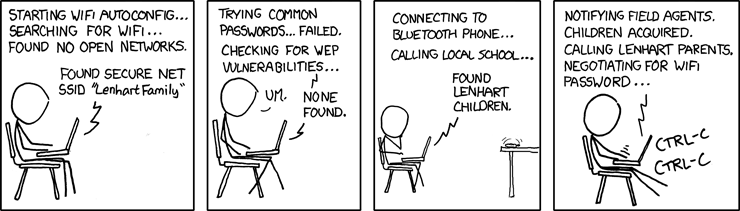
\includegraphics[width=\textwidth, keepaspectratio]{img/xkcd/zealous_autoconfig.png}
	\caption*{{\small \textit{I hear this is an option in the latest Ubuntu release. (https://xkcd.com/416)}}}
\end{figure}

\minisec{University groups}
\label{sec:hsg}

Learning and partying are not enough for you? Find a university group! There you will find volunteer students who want to actively shape life on campus. And depending on what you are looking for, you will also be able to find discussions, the opportunity to help others, new experiences, interesting people and much more.

Thematically, there is something for everyone. There are university groups with political and social commitment. Others are interested in shaping cultural diversity in Dresden. Of course, there are also technically oriented university groups. Just have a look around here~\link{https://www.stura.tu-dresden.de/hochschulgruppen} and contact the university group of your choice directly. Maybe there is something for you.
Vielleicht ist ja was für dich dabei.

\minisec{Study abroad}

If you have an acute desire to go abroad or an urge to internationalize during your studies, please ask the university's international office or your professor of confidence. Stays abroad can cause side effects. You can ask fellow students about theirs.

In the course of your studies, people will ask you again and again whether you would like to spend one or two semesters abroad.
Now you may ask yourself as an innocent freshman, why do that and why are you coming up with it now?
Die Antwort ist einfach:
The answer is simple:
For one, you can directly improve your language skills, socialize and experience new cultures -- A welcome change to clear your head after the exhausting semesters. It gives you new perspectives, both academic and professional. It also helps you develop your soft skills such as independence, tolerance, and adaptability (to name a few). All things that will help you and you will be grateful for later on.
In short, a stay abroad is useful, but requires some planning.
Therefore it is advantageous to inform yourself as early as possible.
For information and if you have any questions, you can contact the International Office (AAA) of the TU~\link{https://tu-dresden.de/studium/im-studium/beratung-und-service/akademisches-auslandsamt} and visit the pages of the faculty~\link{https://tu-dresden.de/ing/informatik/studium/internationales/outgoing}.
If you are brave, you can even ask professors directly if they have contacts to other universities or companies.
It's up to you how successful your stay abroad will be.
Whether it's petting seals off Newfoundland or attending a scrum meeting in Silicon Valley, there are plenty of offers waiting for you!

% \begin{figure}[b!]
% 	\centering
% 	\includegraphics[width=0.9\linewidth]{img/ese2014/einschreibung.jpg}
% \end{figure}%

\minisec{Leave of Absence}
There are a number of reasons that can prevent you from properly continuing your studies at the TU. Classic reasons are serious illnesses, longer internships, stays abroad or (unexpected) offspring that you have to take care of. In such cases, you can take a leave of absence from your studies in order to fully concentrate on the reason for your leave. During a semester of leave, you are exempt from having to take exams, but you continue to enjoy all the benefits of being a student. On the other hand, you are usually not entitled to BAföG or child benefit payments during this time, so don't necessarily plan for this in your income.

If you study abroad and spend a few semesters in far-away countries, you can have your achievements and exams credited here. The only pitfall is that if you earn enough credits, you will still be advanced by one semester, but the student advisor can help you with that.

You can apply for a leave of absence at the Immatrikulationsamt~\link{https://tu-dresden.de/imma/} during the re-registration period for the next semester. You can find out exactly how to do this and further information under~\link{https://tu-dresden.de/studium/im-studium/studienorganisation/beurlaubung}.

% toggles back at the end of this file!
\changemenucolor{gray}{bg}{named}{ese_bg_color} %background of the menukeys
\changemenucolor{gray}{br}{named}{ese_fg_color} %border of the menukeys
\changemenucolor{gray}{txt}{named}{ese_fg_color} %text of the menukeys

\newcommand{\semester}[1]{\minisec{\Large\vspace{.7\baselineskip} #1 Semester\\[.6\baselineskip]}}
\newcommand{\modul}[1]{\vspace{.5\baselineskip}\textbf{\menu[;]{#1\,}}\\[.2\baselineskip]}

\chapter{Module overview}

Here you will find a short overview of the modules you will attend during your studies. The order is not binding, it is only the recommended path through the program.
The symbols \textbf{\menu[;]{I;M;D}} indicate the modules for Bachelor of Computer Science, Bachelor of Media Informatics and Diploma of Computer Science respectively.

\vspace*{-1em}

\semester{1st}

\modul{I; M; D; Einführung in die Mathematik für Informatiker}
You know your way around matrices?
Then you know what to do with the terms determinant, diagonalizability, scalar product and the solution of a homogeneous linear system of equations -- if not, then you will learn it here from scratch.
In addition, in discrete mathematics, the times and pluses are virtually redefined and you learn to think a little differently.

\modul{I; M; D; Algorithmen und Datenstrukturen}
\label{sec:aud}
What comes first?
5 or 3?
Such questions will keep you busy in Algorithmen und Datenstrukturen as you learn about quicksort, heapsort and the like.
% Der Wortwitz gefällt mir...
You will also try your hand at gardening, growing AVL and other trees.
In the process, you will get acquainted with the C programming language.

\modul{I; M; D; Einführungspraktikum}
Have you always loved playing with Lego?
Then you will like this internship, which takes place during the lecture-free period.
As part of a team, you will be given the task of teaching a self-designed robot in Python how to find its way around a maze on its own.
In the process, and in the competition that follows, there is no shortage of fun.
For diploma students, there is an additional one-week individual project, the so called Strategiespiel internship, where you can show what you've got in C or optionally C++. If necessary this internship can be postponed to the summer semester.
In recent years, participants had to write an artificial intelligence for a predetermined well-known board game

\newpage

\modul{I; M; Einführung in die Medieninformatik}
\label{lec:emi}
In this module you will learn how human perception works and how you can design software ergonomically.
In addition, you will be introduced to various properties of information and data formats based on the media comprising text, images, audio and video.
In the section about texts and images, the corresponding document formats of the Internet (HTML and SVG) will be discussed.
You can also expect a short excursion into app development.
Another part of the module gives an overview of document processing using XML techniques.
In tutorials and in the form of a project in a small group over the course of the semester, you will have the opportunity to put what you have learned directly into practice.

\modul{D; Technische Grundlagen und Hardwarepraktikum}
If you've always wanted to know what the electrons in your home computer have to go through, you'll learn exactly that here.
Initially you will look at transistor, diode and operational amplifier circuits.
Based on this, you will take a closer look at logic elements and complex circuits.
In the following semester, you will be able to apply all that you have learned here to plug together a few circuits yourself.

\modul{D; Rechnerarchitektur}
This is about the basic building blocks of a computer:
Memory, bus systems, arithmetic and control units.
Read binary code? All nonsense! In this module you will learn what machine language really looks like and get a crash course in assembler.
You'll also look at the pipelining principle and be confronted with the problems that arise with it.
Finally, we will discuss which methods you can use to accelerate today's computer architectures and to use parallel architectures.

\vfill

\begin{figure}[h!]
\centering
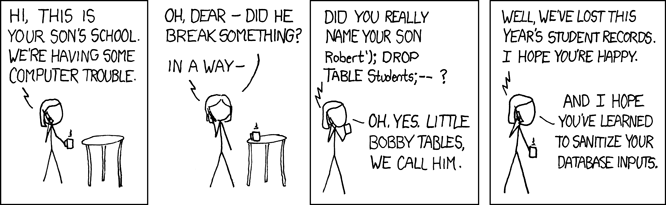
\includegraphics[scale=.5]{img/xkcd/exploits_of_a_mom.png}
\caption*{{\small \textit{Her daughter is named Help I'm trapped in a driver's license factory. (https://xkcd.com/327)}}}
\end{figure}

\semester{2nd}

\modul{I; M; D; Mathematische Methoden für Informatiker}
After the a-level material has sunk in much deeper than before, the next two semesters will take you into new areas of mathematics.
Initially, you'll study the different types of algebraic structures (which are sets of arbitrary symbols and arithmetic operations declared on them).
Vectors, matrices, and fields follow.
Then comes a jump from the discrete to the continuous.
Calculus is not as boring as in school, there is also a version with multiple variables.
The whole thing culminates in the introduction of differential equations.
Towards the end you turn again to polynomials.
First, efficient approximation methods are dealt with, later a short excursion into stochastics ensues.

\modul{I; M; D; Programmierung}
You probably already knew that programming languages don't grow on trees, but here you will learn that they follow strict mathematical rules.
Using a part of the programming language C as an example, the syntax is first defined with the help of grammars.
Shortly after, you will come into contact with the functional programming language Haskell and get to know a completely new approach to programming.
Through many nice, recursively nested mappings, the semantics is then defined, i.e.\ the effect that such a program has on an (abstract) computing machine.
In addition, you will learn how to formally prove the correctness of a program fragment.

\modul{I; M; D; Softwaretechnologie}
Developing software is an art and writing good software is not an easy thing -- if you haven't already -- you will realize this once you reached this module.
To be able to demonstrate this skill, you need some tools of the trade, which you will get here.
You will be introduced to helpful concepts through Java and design procedures alongside professional documentation.
This will lay the foundation for the project in the third semester, where you can earn laurels in project management and software development.


\newpage

\modul{I; D; Informations- und Kodierungstheorie}
What information actually is and what constitutes it will occupy you here.
At the beginning, the focus is on how you can represent and store information.
A little later, it will be explained to you why and how the information is protected by means of coding, so that it arrives at you safely when it is exposed to interference and manipulation on the way.
The knowledge you have acquired in mathematics so far will be of use to you.

\modul{I; Einführung in die Computergraphik}
\label{lec:ecg}
What is actually behind the Unreal Engine? How do shaders work?
Why do the characters in computer games look more and more realistic?
You'll find out in this module, along with the structure of graphics systems, color spaces, raster graphics and their applications.
Existing problems such as aliasing and artifacts are included, as well as their algorithmic solutions.
C++ is used as the programming language for the exercises.

\modul{M; Grundlagen der Gestaltung}
In this module you will learn terminology and general principles of design.
The course is deliberately limited to two-dimensional areas.
Form categories, contrast formation and color theory form the main focus.
The accompanying exercises are designed to give you an insight into the subject matter and to awaken your sensitivity through manual work.

\modul{M; Medien und Medienströme}
Here you will learn about media, their compression and editing.
The application of various tools for the creation of media and their characteristics are also the subject of this course.
Thus, you will deal with the basics of image, audio and video processing in the form of exercises.

\modul{D; Rechnerarchitektur}
Continuation of the 1st semester.

\modul{D; Technische Grundlagen und Hardwarepraktikum}
Continuation of the 1st semester. Circuit diagrams and physical laws -- all well and good. But how does it all fit together?
That's what this module is all about. In a series of experiments, you'll put everything you've learned into practice.
From analog to digital to your own little computer, everything is included!

\newpage

\semester{3rd}

\modul{I; M; D; Mathematische Methoden für Informatiker}
Continuation of the 2nd semester.

\modul{I; M; D; Softwaretechnologie-Projekt}
The project takes up most of the third semester.
Here you have to put your knowledge from the course \enquote{Softwaretechnologie} into practice.
In a team of five you have the task to write an application for a real clientele or the chair.
As a team, you will have to take care of the conception, planning, programming and division of labor.
You consult with the clientele and/or the supervisors and maybe you have to change everything again.
The module ends with the presentation of the finished product.
At the end you will have an impression of what working in IT can look like.

\modul{I; M; D; Formale Systeme}
True?
And or false?
What is false becomes, if it is false false, true?
Logical!
If everyone has an umbrella tomorrow, will it rain?
Besides propositional logic, this module teaches you the basics of formal languages.
This is followed by thoughts on machine computability and automata theory.
Turing sends his regards.

\modul{I; M; Rechnerarchitektur}
See 1st semester for description.

\modul{I; Technische Grundlagen und Hardwarepraktikum}
See 1st semester for description.

\modul{M; Einführung in die Mediengestaltung}
The lecture will teach you the basics of multimedia design from the point of view of the development of individual directions (film, Internet) with reference to the design changes in the past centuries (book).
In addition, you will learn the useful method of metaphor formation and key aspects of interface design.

\newpage

\modul{D; Grundlagen des Nebenfachs}
Depending on which minor you choose, you will deal with topics that are only remotely related to computer science.
Think outside the box and get to know other worlds is the motto.
Here you have the opportunity to get to know students from other disciplines.

\modul{D; Betriebssysteme und Sicherheit}
In this course, you'll take a close look at the servant spirits that toil between the hardware and the colorful applications.
Why can you use a computer to write text, compile code, edit an image, and listen to music all at the same time?
How is your data protected in computer systems?
Why are so many people into this Unix here?

\semester{4th}

\modul{I; M; D; Datenbanken und Rechnernetze}
Where do you put your 20 terabytes of user data? And how does the YouTube video actually get from the USA to your browser?
This is the topic of this module, which consists of two different courses.
In \textit{Datenbanken} you will first learn methods for efficient data storage.
After that, you will be taught how to design and create complex relational databases yourself.
In \textit{Rechnernetze} you will start with the working principles of modems and network cards and you will get a short overview of modern communication and switching protocols.
Also the sector of mobile communication and the difficulties that arise in it are briefly examined.

\modul{I; M; Rechnerarchitektur}
Continuation of the 3rd semester.

\modul{I; D; Theoretische Informatik und Logik}
The continuation of Formale Systeme.
Thus, you consider the correctness and scheduling of algorithms and their necessary effort in terms of time and space requirements.
A detour into predicate logic and logic programming rounds off the module.

\modul{I; Technische Grundlagen und Hardwarepraktikum}
Continuation of the 3rd semester.

\modul{M; Medienpsychologie und -didaktik}
Mediendidaktik is the \enquote{art of teaching}.
Here you will find answers to the questions:
What is education?
How does it proceed?
How can it be improved?
You will learn about the development of teaching methods.
In the parallel internship, you will apply what you have learned to the development of an educational game.

\modul{M; Informations- und Kodierungstheorie}
See 2nd semester for description.

\modul{M; Einführung in die Computergraphik}
See 2nd semester for description.

\modul{M; Medieninformatik-Projekt}
The big highlight of Medieninformatik in the bachelor's degree.
In small groups you have to realize a mobile game, an internet page or something else multimedia.
Apart from the task, there are virtually no limits to your imagination.
It's all about hard work, team spirit and dealing with sleep deprivation when the deadline finally approaches.

\modul{D; Grundlagen des Nebenfachs}
Continuation of the 3rd semester.

\modul{D; Allg. Basisqualifikationen}
English is the only relevant language for computer science.
Here you will learn how to express yourself professionally in English.
If you are already satisfied with your English skills, you can alternatively attend another language course or any course from the university-wide Studium Generale program.
In addition to the two compulsory language courses, there is also a proseminar.
There you will learn \textit{how} to prepare a scientific publication -- by writing and presenting one yourself on a topic of your choice.

\modul{D; Forschungslinie}
Here you will get an overview of current research topics and learn how to work in a research-oriented way.
This module will help you to choose the right specialization later on. Attending this course is also interesting for bachelor's and master's students, as they also have to deepen their knowledge eventually.

\begin{figure}[b!]
\centering
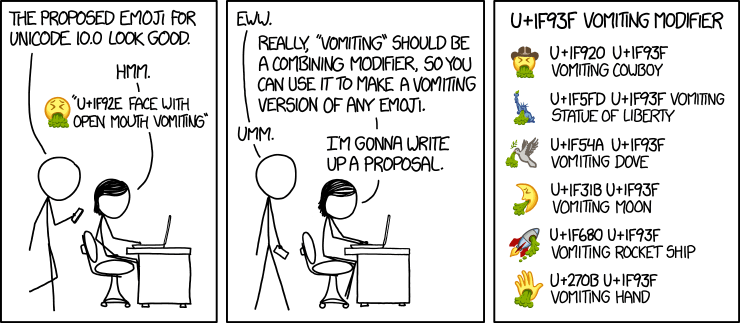
\includegraphics[scale=.4]{img/xkcd/vomiting_emoji.png}
\caption*{{\small \textit{My favorite might be U+1F609 U+1F93F WINKING FACE VOMITING\@. (https://xkcd.com/1813)}}}
\end{figure}
\pagebreak
\semester{5th}

\modul{I; M; Vertiefung in der Informatik/Medieninformatik}
Here you can choose suitable events from a catalog of courses to broaden your scientific horizons.
The options include lectures, tutorials, internships, excursions, seminars and more.

\modul{I; M; Betriebssysteme und Sicherheit}
See 3rd semester for description.

\modul{I; D; Intelligente Systeme}
This module is about artificial intelligence.
Here you will learn problem solving, knowledge representation, planning, and language processing.
Why could IBM's Watson win in \textit{Jeopardy!} against the best human gamers?
How does a spam filter know what is spam and what is not?
You'll learn the answers with the learning algorithms used to find them.

\modul{I; D; Systemorientierte Informatik/Hardware Software Codesign}
This module deals with interfaces between computers and industrial systems.
First, you will abstract what is common to all systems encountered, and terms such as \enquote{system}, \enquote{signal}, and \enquote{control loop} will be formalized to make it easier to work computationally.
You will be made fit for analyzing and predicting transmission behavior and responses that such a system will exhibit given a particular input.
Aspects of audio and video technology such as digitization and filtering are also covered.

\modul{M; Web- und Multimedia Engineering}
How can you make the web multimedia and interactive with today's technology? Why is HTML5 so great?
How do you use professional development tools and appropriate languages to project your imagination into the result?
This module helps to learn appropriate methods and gain experience in using them.

\modul{M; Medieninformatik-Projekt}
Continuation of the 4th semester.

\modul{D; Vertiefung im Nebenfach}
Now that you've learned the basics of your chosen minor, it's time to get serious and dig deeper.

\modul{D; Basismodul 1, 2 und 3}
Here you choose three of seven different topics and deal with them.
You can choose between Applied Computer Science, Artificial Intelligence, Software and Web Engineering, System Architecture, Computer Engineering, Theoretical Computer Science and Computer Graphics.
Within these directions, you can choose suitable courses.

\semester{6th}

\modul{I; M; Spezialisierung in der Informatik/Medieninformatik}
Further in-depth study following the same pattern as in the fifth semester in preparation for the bachelor thesis.

\modul{I; M; Überfachliche Qualifikation}
\label{lec:aqua}
In this type of minor, you'll orient yourself to topics of your interest across disciplines to develop subject-specific expertise.
Plus, this module is another good time to learn a new language. Japanese? Arabic? Russian? Or English again?
Again, courses can be chosen from a catalog.

\newpage

\modul{I; M; Bachelorarbeit und Kolloquium}
As a crowning finale, you will complete your Bachelor's thesis on a topic of your choice and defend it in a presentation.
Congratulations! You are now officially \textit{Bachelor of Science}! How about a Master's degree afterwards?

\modul{D; Vertiefung im Nebenfach}
Continuation of the 5th semester.

\modul{D; Basismodul 1, 2 und 3}
Continuation of the 5th semester.

\semester{7th\ to 10th}

In the computer science diploma program, you have four more semesters to go after the first six. At the same time, most bachelor's students will choose a master's program.
During the seventh semester, you will complete a professional internship, which is also an ideal opportunity for a stay abroad.
In the eighth and ninth, you will then select modules that interest you, descend deeper into the abysses of your chosen topic, acquire further skills according to the same principle as in \enquote{Allgemeine Basisqualifikationen}, write a \enquote{Großen Beleg} (comparable to the bachelor's thesis) and complete further work.
And in the tenth, last semester you finally write your diploma thesis and that's it!
That's how fast it can go.

\begin{figure}[b!]
\centering
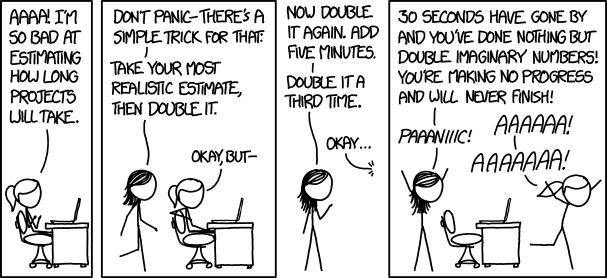
\includegraphics[width=.73\textwidth]{img/xkcd/estimating_time.png}
\caption*{\centering {\small \textit{Corollary to Hofstadter's Law: Every minute you spend thinking about Hofstadter's Law is a minute you're NOT WORKING AND WILL NEVER FINISH\@! PAAAAAANIIIIIIC\@! (https://xkcd.com/1658/)}}}
\end{figure}

\changemenucolor{gray}{bg}{named}{ese_fg_color} %background of the menukeys
\changemenucolor{gray}{br}{named}{ese_bg_color} %border of the menukeys
\changemenucolor{gray}{txt}{named}{ese_bg_color} %text of the menukeys


\includegraphics[height=\pageheight, width=\pagewidth]{img/filmwerbung.jpg}
%\cleardoubleevenemptypage

% ensure we are on a double page
\ifcase\numexpr \modulo{\value{page}}{2} \relax
% don't add any extra pages
\or
\hbox{}
\vspace{5mm}
\begin{center}
\tiny
--- This page is unintentionally left blank ---
\vfill
:P
\end{center}
\newpage
\fi

\addchap[Campusplan]{}
\thispagestyle{empty} %keine Seitenzahl
\AddToShipoutPicture*{\put(0,0){%
\parbox[b][\paperheight]{\paperwidth}{%
\vfill
\centering
\adjincludegraphics[height=\pageheight,keepaspectratio,trim={0 0 {.5\width} 0},clip]{img/campusplan_highlighted.pdf}%
\vfill
}}}
\mbox{}
\newpage
\thispagestyle{empty} %keine Seitenzahl
\AddToShipoutPicture*{\put(0,0){%
\parbox[b][\paperheight]{\paperwidth}{%
\vfill
\centering
\adjincludegraphics[height=\pageheight,keepaspectratio,trim={{.5\width} 0 0 0},clip]{img/campusplan_highlighted.pdf}%
\vfill
}}}
\mbox{}


\end{document}
